\documentclass[a4paper,11pt]{article}

% --- Geometry & Spacing (brief: 2--2.5cm margins, 1.1x line spacing) ---
\usepackage[margin=2.2cm]{geometry}
\usepackage{setspace}
\setstretch{1.1}

% --- Fonts (brief: Helvetica / Arial family, 11pt body) ---
\usepackage[T1]{fontenc}
\usepackage{helvet}
\renewcommand{\familydefault}{\sfdefault}
\usepackage{microtype}
\usepackage{amssymb}
\usepackage{xcolor}

% --- Prevent orphan headings / widows ---
\widowpenalty=10000
\clubpenalty=10000
\raggedbottom

% --- Graphics, diagrams, PDF embedding ---
\usepackage{tikz}
\usetikzlibrary{shapes,shapes.geometric,shapes.symbols,arrows.meta,positioning,calc,fit,decorations.pathreplacing}
\usepackage{graphicx}
\usepackage{pdfpages}
\usepackage{pdflscape}
\usepackage{adjustbox}
\usepackage{float}

% --- Tables & Lists ---
\usepackage{array}
\usepackage{booktabs}
\usepackage{longtable}
\usepackage{enumitem}

% --- Headers & Page Numbers (brief: pages must be numbered) ---
\usepackage{fancyhdr}
\pagestyle{fancy}
\fancyhf{}
\fancyfoot[C]{\thepage}
\renewcommand{\headrulewidth}{0pt}

% --- Hyperlinks & PDF bookmarks ---
\usepackage[hidelinks,bookmarks=true,pdfusetitle]{hyperref}

% --- Referencing: Harvard style (brief requirement) ---
\usepackage[style=authoryear,backend=biber]{biblatex}
\addbibresource{references.bib}

% --- Word-count helper macro (visual reminder only; not enforced) ---
\newcommand{\wclimit}[1]{\hfill\textit{\footnotesize(max #1 words)}}

\newcommand{\MYhref}[3][blue]{\href{#2}{\color{#1}{#3}}}%

% ============================================================
\begin{document}

% --- Cover Page (brief: Name, Module code & Year, OneDrive URL, ToC) ---
\begin{center}
    \vspace*{3cm}
    {\LARGE\bfseries StudyBuddy\par}
    \vspace{0.4cm}
    {\Large CW2 Report\par}
    \vspace{1.5cm}
    {\large IN3065 User-Centred System Design 2025--2026\par}
    \vspace{1cm}
    {\large Anker Rasmussen \\230022888\par}
    \vspace{1.5cm}
    {\normalsize Raw data (interview recordings):
    \MYhref{https://cityuni-my.sharepoint.com/:f:/g/personal/anker_rasmussen_city_ac_uk/IgDGVR9azIIOTK3t1XU7LSTyAUYfGKY0C_x_EShOPKYeH2k?e=O9kAHL}{OneDrive folder (City login required)}\par}
    \vfill
\end{center}
\newpage
\tableofcontents
\vspace{2cm}

% ============================================================
% SECTION 1: USER RESEARCH
% ============================================================
\newpage
\section{User Research}
\subsection{User Research Methodology}\label{sec:methodology}
\wclimit{250}

Four semi-structured interviews were conducted with potential users
of StudyBuddy: undergraduate Y2 Electrical Engineers enrolled on the
same semester-2 module set (mechatronics, engineering design,
sensors \& instrumentation, data analysis, engineer in society).

Recruitment used a five-question Qualtrics prescreening survey
(Appendix~\ref{app:research-materials}) with inclusion criteria:
(i)~current undergraduate or postgraduate study; (ii)~regular study
outside contact hours; (iii)~use of third-party tools beyond Moodle,
course textbooks, and OneDrive; and (iv)~availability for a
${\sim}20$-minute interview. Criterion~(iii) deliberately biased
recruitment towards students who already supplement Moodle with
personal tooling. This is the population StudyBuddy is positioned to
support.

Interviews ran 20--30 minutes each, in person, semi-structured, and
video-recorded with participants' faces shown. Recordings were
transcribed via Teams' auto-transcript function and cleaned to
markdown. All four interviews included a walkthrough segment, in
three different forms: live screen-share of a study setup (P1, P4);
demonstration of physical artefacts, including a wall-mounted
colour-coded formula corkboard (P2); and a brief verbal
scenario walkthrough of a pre-exam study session (P3, less in-depth
than the other three, with no live setup or artefact shown).

Ethics followed the module template: informed consent forms
collected real names and University email addresses, and a
Participant Information Sheet was provided. Participants were
anonymised to P1--P4 at the cleaning stage; the four signed
consent forms are submitted as the separate \emph{Signed Informed
Consent Forms} PDF, per the coursework brief.

Analysis followed \textcite{braun2006}'s reflexive thematic
analysis: familiarisation, line-level open coding
(Appendix~\ref{app:analysis}), affinity-style clustering into
candidate themes, review against data extracts, and final theme
definition. Walkthrough observations are reported separately as
descriptive records (Appendix~\ref{app:observation}).
\subsection{User Research Results}\label{sec:results}
\wclimit{600}

\subsubsection*{Participants}

Four undergraduate engineering students at City University, on
a shared semester-2 module set.\\ \textbf{P1}: NotebookLM and Notion
user; fixed 20:00--23:00 evening study block; live walkthrough.
\\ \textbf{P2}: heavy hand-writing practice with a wall-mounted formula
corkboard; refuses evening study; single desk shared with gaming PC;
artefact-only walkthrough.\\ \textbf{P3}: late-night bedroom study to
avoid family activity; minimal tooling; brief verbal walkthrough
only (no live setup or artefact).
\\ \textbf{P4}: multi-monitor setup with an iPad subject/exam/topic
folder hierarchy; leaves home for serious coursework; live walkthrough.

\subsubsection*{Key Findings}

\textbf{T1: ``Which equation?''}\quad The dominant cognitive
bottleneck is selecting \emph{which} equation to apply, not arithmetic
(P2, line~77; P3, line~57). The most-wanted artefact is a
step-by-step worked solution. Where Moodle provides only numerical
answers (``560 kg for mass'' P1, line~263) or releases solutions
a week late (P4, line~159), participants cascade through
nearest-similar tutorial $\rightarrow$ AI $\rightarrow$ YouTube
$\rightarrow$ pre-exam peer help. AI use is trust-bounded by an
explicit fear of ``AI getting the calculation totally wrong, showing
you the right result, but not the right way to get there'' (P2,
line~169).

\textbf{T2: Prioritisation is personal and rarely tracked.}\quad
Each participant uses a different primary rule: difficulty (P1),
session-count goals (P2), deadline (P3), motivation (P4). Time-of-day
preferences are mutually incompatible (20--23h, 14--16h, 22--24h,
timetable-gap-only). No participant plans more than ${\sim}3$~days
ahead or tracks progress beyond mental goals. Effort, not output, is
the implicit success metric (P2, line~285).

\textbf{T3: Focus is engineered, not willed.}\quad All four
participants enter focus through deliberate spatial (bedroom-vs-living-room),
temporal (time-of-day), and physical (keyboard relocation, single
earbud, formula corkboard, multi-monitor) levers. Default willpower is not
the strategy.

\textbf{T4: Group study is exam-shaped, ad-hoc, brittle.}\quad All
four use group study, only as exams approach, coordinated spontaneously
(``@everyone, who wants to join?''), and vulnerable to off-topic
chatter and pace mismatch (P1, line~205). It nonetheless performs two
real functions: screen-shared problem solving (a substitute worked
example) and explain-to-learn (P4, line~247).

\textbf{T5: Moodle is a delivery channel, not a study artefact.}\quad
All four treat Moodle as the inescapable on-ramp, but each builds a
separate personal external memory beside it, in very different forms
(Notion + NotebookLM; hand-written colour-coded notes plus a formula corkboard;
iPad folder hierarchy; ad-hoc downloads). Friction is
unevenly perceived but the underlying pattern is uniform.

\subsubsection*{Design Goal}

Address the \textbf{worked-example gap (T1)} and the
\textbf{personal, short-horizon prioritisation pattern (T2)} that
determines when and on what these students actually revise, for
second-year undergraduates revising quantitative engineering
modules. Specifically: surface step-by-step worked solutions and
AI procedure explanation with hallucination guardrails (T1),
delivered to fit each student's own prioritisation rule and ad-hoc,
deadline-driven rhythm rather than imposing a long-horizon study
plan (T2), and \emph{coexisting with} (rather than replacing) the
personal external memory each student has already built (T5).

\subsubsection*{Key Requirements}

R1--R10, summarised below; full descriptions with finding-level
tagging are in Appendix~\ref{app:requirements}. R-IDs are
referenced inline on each wireframe annotation panel
(\S\ref{sec:wireframes}).

\begin{itemize}[leftmargin=2.4em,itemsep=1pt]
  \item[\textbf{R1}] Tomorrow's class card on the home screen. [T1, T2]
  \item[\textbf{R2}] One-paragraph last-session recap, terms deep-linked to slides. [T1]
  \item[\textbf{R3}] Sourced step-by-step worked solutions before any AI text. [T1]
  \item[\textbf{R4}] Past papers and mocks as a first-class source. [T1]
  \item[\textbf{R5}] Coexist with Moodle, MyTimetable and a notes provider. [T5]
  \item[\textbf{R6}] Paper or file capture into the worked-solution flow. [T1]
  \item[\textbf{R7}] Informal, deadline-driven rhythm; no streaks or long-horizon plans. [T2]
  \item[\textbf{R8}] Plan rows show \emph{what}, \emph{why this size}, \emph{when due}. [T2]
  \item[\textbf{R9}] Adapt to the student's chosen prioritisation rule. [T2]
  \item[\textbf{R10}] Capture felt-readiness per topic at wrap-up. [T2]
\end{itemize}

\newpage
\begin{landscape}
\subsection{Current User Journey Map}\label{sec:journey}

\begin{figure}[!ht]
\centering
\definecolor{jmInk}{HTML}{1F2933}
\definecolor{jmMid}{HTML}{52606D}
\definecolor{jmSoft}{HTML}{EEF1F4}
\definecolor{jmLine}{HTML}{CBD2D9}
\definecolor{jmAcc}{HTML}{2667FF}
\definecolor{jmPain}{HTML}{C2410C}
\definecolor{jmGood}{HTML}{0B7A55}
\definecolor{jmBg}{HTML}{F8F9FB}

% --- Layout constants (used by tikzpicture, in cm) ---
\newcommand{\jmLW}{2.6}      % row-label column width
\newcommand{\jmCW}{4.0}      % phase column width
\newcommand{\jmRH}{2.0}      % data row height
\newcommand{\jmHH}{0.9}      % header row height
% Cell text width = column width minus 0.4cm padding, in *current* dim.
\newcommand{\jmCellTextW}{\dimexpr\jmCW cm-0.4cm\relax}

% --- Cell helper ---
% args: #1 = column index (1..6); #2 = row index (1..5); #3 = body
\newcommand{\jmcell}[3]{%
  \node[cell, minimum width=\jmCW cm, minimum height=\jmRH cm,
        anchor=north west, text width=\jmCellTextW,
        font=\sffamily\scriptsize, align=left]
    at ({\jmLW + (#1-1)*\jmCW},{-\jmHH - (#2-1)*\jmRH}) {#3};%
}

\resizebox{\linewidth}{!}{%
\begin{tikzpicture}[
    every node/.style={font=\sffamily,inner sep=0pt, text=jmInk},
    cell/.style={
        rectangle, draw=jmLine, line width=0.3pt, fill=white,
        align=left, inner sep=4pt, text=jmInk,
    },
    rowlabel/.style={
        rectangle, fill=jmSoft, draw=jmLine, line width=0.3pt,
        align=center, inner sep=4pt, font=\sffamily\bfseries\footnotesize,
        text=jmMid,
    },
    phasebox/.style={
        rectangle, fill=jmInk, draw=jmInk,
        align=center, inner sep=5pt,
        font=\sffamily\bfseries\footnotesize, text=white,
    },
]

% --- Header row (phases) ---
\foreach \i/\name in {1/Decide,2/Gather,3/Set up,4/{Get into it},5/Study,6/{Wrap up}} {
    \node[phasebox, minimum width=\jmCW cm, minimum height=\jmHH cm,
          anchor=north west]
        at ({\jmLW + (\i-1)*\jmCW},0) {\name};
}
\node[rowlabel, minimum width=\jmLW cm, minimum height=\jmHH cm,
      anchor=north west]
    at (0,0) {Phase};

% --- Row labels ---
\foreach \r/\lab in {1/Actions, 2/Thoughts, 3/Emotions,
                     4/{Pain points}, 5/Opportunities} {
    \node[rowlabel, minimum width=\jmLW cm, minimum height=\jmRH cm,
          anchor=north west]
        at (0,{-\jmHH - (\r-1)*\jmRH}) {\lab};
}

% --- Row 1: Actions ---
\jmcell{1}{1}{Open Moodle on the laptop. Check what was uploaded today.
\,[P1~I1:109]}
\jmcell{2}{1}{Download tutorial sheet + lecture slides. Open both in
side-by-side tabs / monitors. \,[P2~I2:315], [P4~I4:189]}
\jmcell{3}{1}{Move keyboard aside; put one earbud in; move from
living room to bedroom. \,[P1~I1:153], [P2~I2:205]}
\jmcell{4}{1}{Re-read previous session's notes on a second monitor or
iPad. \,[P4~I4:259]}
\jmcell{5}{1}{Attempt the question. Get stuck. Try nearest tutorial,
then AI, then YouTube. \,[P1~I1:255], [P4~I4:313]}
\jmcell{6}{1}{Close laptop; mark a vague mental tick.
``Sessions 1 and 2 done.'' \,[P2~I2:281]}

% --- Row 2: Thoughts ---
\jmcell{1}{2}{``What's due first? What's hardest right now?'' \,[F18]}
\jmcell{2}{2}{``Is the answer key actually here, or just
`560\,kg for mass'?'' \,[P1~I1:263]}
\jmcell{3}{2}{``I need to actually be in studying mode before this
counts.'' \,[P1~I1:181]}
\jmcell{4}{2}{``Where was I last time? What was the topic?''
\,[P4~I4:259]}
\jmcell{5}{2}{``Which equation goes here? The lecture didn't actually
show the steps.'' \,[P2~I2:77,~311]}
\jmcell{6}{2}{``If I worked hard, that's a good day, even if I didn't
finish.'' \,[P2~I2:285]}

% --- Row 3: Emotions ---
% Six tinted backing cells.
\foreach \i in {1,...,6} {
    \node[cell, minimum width=\jmCW cm, minimum height=\jmRH cm,
          anchor=north west, fill=jmSoft]
        at ({\jmLW + (\i-1)*\jmCW},{-\jmHH - 2*\jmRH}) {};
}

% Emotion plot. Coordinates are explicit cm pairs.
% Centre of the emotion row (y), and column centres (x).
\draw[jmAcc, line width=1.0pt]
    plot[smooth, tension=0.55] coordinates {
        ({\jmLW + 0.5*\jmCW},{-\jmHH - 2.5*\jmRH + 0.0})
        ({\jmLW + 1.5*\jmCW},{-\jmHH - 2.5*\jmRH - 0.35})
        ({\jmLW + 2.5*\jmCW},{-\jmHH - 2.5*\jmRH + 0.0})
        ({\jmLW + 3.5*\jmCW},{-\jmHH - 2.5*\jmRH + 0.4})
        ({\jmLW + 4.5*\jmCW},{-\jmHH - 2.5*\jmRH - 0.85})
        ({\jmLW + 5.5*\jmCW},{-\jmHH - 2.5*\jmRH + 0.25})
    };

% Emotion dots + labels (explicit, no foreach).
\foreach \i/\dy/\lab in {
    1/0.0/{neutral},
    2/-0.35/{Moodle friction},
    3/0.0/{re-prime},
    4/0.4/{warm-up},
    5/-0.85/{stuck on equation},
    6/0.25/{``effort done''}%
} {
    \fill[jmAcc] ({\jmLW + (\i-0.5)*\jmCW},{-\jmHH - 2.5*\jmRH + \dy}) circle (2.0pt);
    \node[font=\sffamily\tiny, text=jmMid, anchor=south, yshift=4pt]
        at ({\jmLW + (\i-0.5)*\jmCW},{-\jmHH - 2.5*\jmRH + \dy}) {\lab};
}

% --- Row 4: Pain points ---
\jmcell{1}{4}{\textcolor{jmPain}{$\blacktriangledown$~No look-ahead:
plans only 1--3 days out. \,[F21]}}
\jmcell{2}{4}{\textcolor{jmPain}{$\blacktriangledown$~Lecturer-by-lecturer
Moodle layouts; click friction; 300-page monoliths. \,[F42--F44]}}
\jmcell{3}{4}{\textcolor{jmPain}{$\blacktriangledown$~Same machine for
gaming and study creates a context-switch trap. \,[F30]}}
\jmcell{4}{4}{\textcolor{jmPain}{$\blacktriangledown$~Re-entry to last
week's topic is manual; no built-in recap. \,[F24]}}
\jmcell{5}{4}{\textcolor{jmPain}{$\blacktriangledown$~Worked steps
missing; AI hallucinates the working; YouTube is a rabbit hole.
\,[F4, F11, F17]}}
\jmcell{6}{4}{\textcolor{jmPain}{$\blacktriangledown$~No record of what
was actually understood; ``effort'' is the implicit metric. \,[F23]}}

% --- Row 5: Opportunities ---
\jmcell{1}{5}{\textcolor{jmGood}{$\blacktriangle$~Surface ``what's on
tomorrow'' card tied to MyTimetable + Moodle.}}
\jmcell{2}{5}{\textcolor{jmGood}{$\blacktriangle$~Auto-pull tutorial,
slides, past papers into one briefing per class.}}
\jmcell{3}{5}{\textcolor{jmGood}{$\blacktriangle$~Mobile entry point:
glanceable while the laptop is still off.}}
\jmcell{4}{5}{\textcolor{jmGood}{$\blacktriangle$~Pre-loaded recap of
last session, automatically.}}
\jmcell{5}{5}{\textcolor{jmGood}{$\blacktriangle$~Step-by-step worked
solution with sourced citations + AI procedure that names its source.}}
\jmcell{6}{5}{\textcolor{jmGood}{$\blacktriangle$~Capture felt
readiness per topic; feed forward into the next briefing.}}

% --- Decision-point markers (overlay diamonds on the Actions row) ---
\node[diamond, draw=jmAcc, fill=white, line width=0.5pt, inner sep=1pt,
      font=\sffamily\tiny, text=jmAcc, minimum width=0.6cm, minimum height=0.6cm]
    at ({\jmLW + 1*\jmCW},{-\jmHH - 0.5*\jmRH}) {D1};
\node[diamond, draw=jmAcc, fill=white, line width=0.5pt, inner sep=1pt,
      font=\sffamily\tiny, text=jmAcc, minimum width=0.6cm, minimum height=0.6cm]
    at ({\jmLW + 2*\jmCW},{-\jmHH - 0.5*\jmRH}) {D2};
\node[diamond, draw=jmAcc, fill=white, line width=0.5pt, inner sep=1pt,
      font=\sffamily\tiny, text=jmAcc, minimum width=0.6cm, minimum height=0.6cm]
    at ({\jmLW + 5*\jmCW},{-\jmHH - 0.5*\jmRH}) {D3};

% --- Legend node ---
\node[font=\sffamily\scriptsize, text=jmMid, anchor=north west, align=left,
      text width=26.6cm]
    at (0,{-\jmHH - 5*\jmRH - 0.25}) {%
    \textbf{Decision points.}
    \textbf{D1}~Which module first today?
    \,(\emph{rule used differs per participant: difficulty / deadline /
    sessions / motivation; F18}).\quad
    \textbf{D2}~Drip-released today, or wait until everything is up?
    \,(\emph{P4 prefers full upload; F45}).\quad
    \textbf{D3}~Stuck: near-neighbour tutorial $\rightarrow$ AI
    $\rightarrow$ YouTube $\rightarrow$ pre-exam Discord call \,(F9).%
    \par\smallskip
    \textbf{Reading the emotion line.} The blue plot tracks cohort affect
    across the journey. The deepest dip is in the \emph{Study} phase,
    driven by the worked-example gap (T1). Wrap-up rebounds because
    effort, not output, is the felt success metric (T2).%
};

\end{tikzpicture}%
}
\caption{Current user journey map for a typical evening study session,
drawn from P1--P4. Phases run left to right; rows show actions,
thoughts, the affective line (squiggle), pain points (orange) and
opportunities (green). Decision diamonds D1--D3 mark the points where
participants diverge most. Tags refer to interview transcripts
\texttt{[Px Iy:zz]} and findings \texttt{[F\#]} in
Appendix~\ref{app:findings}.}\label{fig:journey}
\end{figure}
\end{landscape}

\clearpage
\subsection{Primary Persona}\label{sec:persona}

The primary persona below (Figure~\ref{fig:persona}) is a single
composite drawn from P1--P4. The method by which it was built
is in \S\ref{sec:persona-method}; every claim on the page is tagged
to a participant or finding so the persona can be audited against
the source data.

\begin{figure}[p]
\centering
\definecolor{personaInk}{HTML}{1F2933}
\definecolor{personaMid}{HTML}{52606D}
\definecolor{personaSoft}{HTML}{E4E7EB}
\definecolor{personaLine}{HTML}{CBD2D9}
\definecolor{personaAcc}{HTML}{2667FF}
\definecolor{personaBg}{HTML}{F8F9FB}

\resizebox{\linewidth}{!}{%
\begin{tikzpicture}[
    every node/.style={font=\sffamily,inner sep=0pt},
    block/.style={
        rectangle, rounded corners=2pt, draw=personaLine, line width=0.4pt,
        fill=white, align=left, inner sep=8pt, text=personaInk
    },
    chip/.style={
        rectangle, rounded corners=3pt, draw=personaLine, line width=0.4pt,
        fill=personaSoft, inner xsep=6pt, inner ysep=3pt,
        outer sep=0pt, minimum height=0.6cm,
        font=\sffamily\scriptsize, text=personaInk
    },
    sectiontitle/.style={
        font=\sffamily\bfseries\footnotesize, text=personaMid
    },
]

% --- Outer frame ---
% Frame height accounts for the tallest natural block (Frustrations,
% which grows past its min-height to fit five bullets):
%   header (3.2) + top gap (0.6) + 3 * \pblockH (17.1) + headroom for
%   over-min growth (~0.4) + 2 * \pblockGap (1.1) + bottom gap (0.6)
%   + footer (1.4) ~= 24.4 cm. Frame set to 25 cm with a small margin.
\node[
    rectangle, draw=personaLine, line width=0.5pt, fill=personaBg,
    minimum width=18.0cm, minimum height=25.0cm, anchor=north west,
] (frame) at (0,0) {};

% --- Header band ---
\node[
    rectangle, fill=personaInk, minimum width=18.0cm, minimum height=3.2cm,
    anchor=north west,
] (header) at (frame.north west) {};

% Avatar circle
\node[
    circle, draw=white, line width=1.2pt, fill=personaAcc,
    minimum size=2.1cm,
] (avatar) at ($(header.west)+(1.6cm,0)$) {};
\node[font=\sffamily\bfseries\Large, text=white] at (avatar) {SA};

% Header text (left block: name + descriptor)
\node[anchor=west, text=white, font=\sffamily\bfseries\LARGE]
    at ($(avatar.east)+(0.6cm,0.55cm)$) {Sam Walker};
\node[anchor=west, text=white, font=\sffamily\small]
    at ($(avatar.east)+(0.6cm,0.0cm)$)
    {Year 2 BEng EEE \,$\cdot$\, City St George's};
\node[anchor=west, text=white!75, font=\sffamily\footnotesize]
    at ($(avatar.east)+(0.6cm,-0.5cm)$)
    {20 y/o \,$\cdot$\, Tube commute \,$\cdot$\, lives at home};

% Tagline / quote (right side of header)
\node[anchor=east, text=white, font=\sffamily\itshape\small,
      align=right, text width=5.4cm]
    at ($(header.east)+(-0.6cm,0)$)
    {``As soon as I don't understand, I just download the solutions
     \dots\ but they give us \emph{560\,kg for mass}.''
     \\[3pt]\textnormal{\textmd{\scriptsize \textendash\ Sam,
     mechatronics tutorial \,[P1~I1:255,~263]}}};

% --- Two-column body ---
% All blocks share the same minimum height so the two columns end at
% the same y. Block-internal padding (inner sep) is generous so the
% bullet text doesn't crowd the rounded borders.
\def\pblockH{5.7cm}    % uniform block height
\def\pblockGap{0.55cm} % vertical gap between blocks in a column

% Left column ----------------------------------
\node[
    block, anchor=north west, text width=7.4cm, minimum height=\pblockH,
    inner sep=12pt,
] (goals) at ($(header.south west)+(0.6cm,-0.6cm)$) {
    \textbf{\sffamily\small Goals}\\[8pt]
    {\footnotesize\sffamily
    $\bullet$~Walk into tomorrow's tutorial knowing
    \emph{which equation to use} on each question.\\[5pt]
    $\bullet$~Spend revision time on the topic that will help most,
    not on whatever opens first.\\[5pt]
    $\bullet$~Keep a personal memory of solved problems that
    survives past exam season.\\[5pt]
    $\bullet$~Pre-empt the panic Discord call by closing the gap
    before the day before the exam.}
};

\node[
    block, anchor=north west, text width=7.4cm, minimum height=\pblockH,
    inner sep=12pt,
] (behaviours) at ($(goals.south west)+(0,-\pblockGap)$) {
    \textbf{\sffamily\small Behaviours}\\[8pt]
    {\footnotesize\sffamily
    $\bullet$~Studies in a fixed evening block, after dinner and a
    \emph{decompression} routine \,[P1~I1:181].\\[4pt]
    $\bullet$~Attempts the tutorial first; downloads the solution
    only on getting stuck \,[P1~I1:255].\\[4pt]
    $\bullet$~Tries to find the link between lecture content and the
    tutorial questions \,[P2~I2:303].\\[4pt]
    $\bullet$~Re-reads the previous session's notes on a second
    screen before starting the next session \,[P4~I4:259].\\[4pt]
    $\bullet$~Joins ad-hoc Discord study calls only as exams approach
    \,[P1~I1:201], [P3~I3:265], [P4~I4:247].}
};

\node[
    block, anchor=north west, text width=7.4cm, minimum height=\pblockH,
    inner sep=12pt,
] (frustrations) at ($(behaviours.south west)+(0,-\pblockGap)$) {
    \textbf{\sffamily\small Frustrations}\\[8pt]
    {\footnotesize\sffamily
    $\bullet$~Numerical-only Moodle solutions: ``560\,kg for mass'',
    no working \,[P1~I1:263].\\[4pt]
    $\bullet$~Tutorial answers released a week late, locking out
    catch-up \,[P4~I4:159].\\[4pt]
    $\bullet$~Each lecturer organises Moodle differently, forcing
    re-orientation \,[P2~I2:145].\\[4pt]
    $\bullet$~Fear of AI returning a correct answer with the wrong
    working \,[P2~I2:169].\\[4pt]
    $\bullet$~Group study slips off-topic or runs at the wrong pace
    \,[P1~I1:205--209].}
};

% Right column ---------------------------------
\node[
    block, anchor=north east, text width=7.4cm, minimum height=\pblockH,
    inner sep=12pt,
] (context) at ($(header.south east)+(-0.6cm,-0.6cm)$) {
    \textbf{\sffamily\small Study context}\\[8pt]
    {\footnotesize\sffamily
    $\bullet$~Same semester-2 module set as P1--P4: mechatronics,
    engineering design, sensors \& instrumentation, data analysis,
    engineer in society.\\[5pt]
    $\bullet$~Studies at a bedroom desk; uses the campus silent room
    between classes \,[P1~I1:161].\\[5pt]
    $\bullet$~Plans 1--3 days ahead at most \,[F21]; tracks progress
    by feel rather than tooling \,[F22].\\[5pt]
    $\bullet$~Time-of-day preference is fixed (one of 14--16h,
    20--23h or 22--24h, depending on living situation) \,[F26].}
};

\node[
    block, anchor=north east, text width=7.4cm, minimum height=\pblockH,
    inner sep=12pt,
] (tools) at ($(context.south east)+(0,-\pblockGap)$) {
    \textbf{\sffamily\small Tools \& tech}\\[8pt]
    {\footnotesize\sffamily
    $\bullet$~Moodle (course gateway, can't be avoided).\\[4pt]
    $\bullet$~Personal external memory: Notion + iPad folders +
    handwritten colour-coded sheets, depending on the student
    \,[F46].\\[4pt]
    $\bullet$~AI (ChatGPT) for procedure explanation;
    NotebookLM only at exam time.
    \,[F10, F13, F14].\\[4pt]
    $\bullet$~YouTube for topic-level understanding, not problem
    solving \,[F16].\\[4pt]
    $\bullet$~Phone always to hand; iPad / second monitor where
    available.}
};

\node[
    block, anchor=north east, text width=7.4cm, minimum height=\pblockH,
    inner sep=12pt,
] (priorities) at ($(tools.south east)+(0,-\pblockGap)$) {
    \textbf{\sffamily\small Prioritisation rule (one of)}\\[10pt]
    \begin{tikzpicture}[every node/.style={font=\sffamily}, inner sep=0pt]
      \node[chip] (r1) at (0,0) {\textbf{Difficulty}};
      \node[chip,right=3pt of r1] (r2) {\textbf{Deadline}};
      \node[chip,right=3pt of r2] (r3) {\textbf{Sessions}};
      \node[chip,right=3pt of r3] (r4) {\textbf{Motivation}};
    \end{tikzpicture}\\[10pt]
    {\footnotesize\sffamily
    Sam picks one and sticks to it. The four rules are mutually
    incompatible across the cohort \,[F18]; StudyBuddy must accept
    whichever Sam chooses, not impose its own \,[T2].}
};

% --- Footer band: themes traced ---
% Footer height bumped to 1.4cm and themes text uses scriptsize so the
% full T1--T5 list fits on one line within 18cm.
\node[
    rectangle, fill=personaSoft, minimum width=18.0cm, minimum height=1.4cm,
    anchor=south west,
] (footer) at (frame.south west) {};
\node[anchor=west, text=personaMid, font=\sffamily\scriptsize\bfseries]
    at ($(footer.west)+(0.55cm,0)$)
    {THEMES TRACED};
\node[anchor=west, text=personaInk, font=\sffamily\scriptsize]
    at ($(footer.west)+(3.6cm,0)$)
    {T1 worked-example gap \,$\cdot$\, T2 personal prioritisation
     \,$\cdot$\, T3 engineered focus \,$\cdot$\, T4 group study
     \,$\cdot$\, T5 external memory};

\end{tikzpicture}%
}
\caption{Primary persona. Sam Walker is a composite drawn from P1--P4,
not any individual participant. Every claim is tagged to evidence
\texttt{[Px Iy:zz]} or to a finding \texttt{[F\#]} in
Appendix~\ref{app:findings}. Themes traced are defined in
\S\ref{sec:results}.}\label{fig:persona}
\end{figure}

\subsubsection{Persona Creation Method}\label{sec:persona-method}

The primary persona was built from the four interview transcripts
following the procedure recommended by \textcite{cooper2014}. After
familiarisation and open coding (Appendix~\ref{app:analysis}), the
five themes T1--T5 (\S\ref{sec:results}) were treated as the core
constraints any persona had to satisfy. A single composite persona
was chosen rather than four individual ones because the cohort
agrees on the design-relevant pattern (the worked-example gap and
short-horizon, personal prioritisation: T1, T2) while disagreeing
on how it shows up day to day (time of day, room, main tooling).
The composite is deliberate: each persona attribute maps either
to a directly observed behaviour, with the participant cited as
\texttt{[Px Iy:zz]}, or to a cohort-wide finding cited as
\texttt{[F\#]} (e.g.\ F18 for the four mutually incompatible
prioritisation rules, F26 for the time-of-day spread). Where
participants diverge, the persona shows that as a chip row rather
than a single value, so the design constraint (``StudyBuddy must
accept whichever rule the student picks'') is on the page rather
than averaged away. Demographics not in the data (name, exact age)
are fictional but plain and clearly marked as such.

% ============================================================
% SECTION 2: DESIGN
% ============================================================
\newpage
\section{Design}

\subsection{Wireframes Intro}\label{sec:wireframes-intro}

The wireframed journey addresses the two dominant findings:
\textbf{T1} (worked-example gap) and \textbf{T2} (personal,
short-horizon prioritisation). It runs from \emph{tomorrow's class
card $\rightarrow$ briefing $\rightarrow$ equation picker
$\rightarrow$ sourced worked solution $\rightarrow$ committed plan
$\rightarrow$ wrap-up}, with a paper-capture flow alongside. Seven
screens rather than six: capture is a separate entry point into the
worked-solution flow, not a step within it, so it gets its own
frame.

\textbf{Mobile-first.}\quad The moments that prompt a check are
quick and unscheduled (what's on tomorrow, snapping a stuck
question, logging felt readiness); none of them need desktop
chrome. The phone is also the only device with a camera in the
student's hand, which is what makes the paper-capture flow workable
(P1~[I1:255], P2~[I2:149], P3~[I3:137], P4~[I4:175]). Longer
focus work hands off to a web companion (out of scope); P4's
multi-monitor habit \mbox{[I4:189--205]} is not well served by a
small screen.

\textbf{Rhythm-agnostic.}\quad The rendered state is for
illustration only; the design adapts to each participant's
prioritisation rule rather than a fixed clock, since time-of-day
preferences are mutually incompatible (T2: 20--23h, 14--16h,
22--24h, timetable-gap-only).

\clearpage
\subsection{Flow Diagram}\label{sec:flow}

Figure~\ref{fig:flow} is the user flow as a standard
flowchart. Terminators (rounded) bookend the session; rectangles are
in-app screen processes and the trapezium is the camera-capture
screen (manual input)~--- together, the seven wireframed screens;
diamonds are user decisions. Two side branches sit off the main
column: a first-run onboarding loop on the right (via \emph{01 Home
empty}), and a paper-capture branch on the left (via \emph{07
Capture}). A return arrow on the far left closes the daily loop:
\emph{End of session} feeds tomorrow's \emph{02 Briefing}, routed
around \emph{07 Capture} so it does not cross any of the in-session
arrows.

\begin{figure}[H]
\centering
\definecolor{flInk}{HTML}{1F2933}
\definecolor{flMid}{HTML}{52606D}
\definecolor{flSoft}{HTML}{EEF1F4}
\definecolor{flLine}{HTML}{CBD2D9}
\definecolor{flAcc}{HTML}{2667FF}
\definecolor{flBg}{HTML}{F8F9FB}
\definecolor{flAlt}{HTML}{C2410C}

\centering
\resizebox{\linewidth}{!}{%
\begin{tikzpicture}[
    >=Stealth,
    every node/.style={font=\sffamily, text=flInk},
    % Standard flowchart shapes (BS 4058 / ISO 5807 conventions):
    %   - Terminator (start / end):  rounded rectangle (pill)
    %   - Process (screen step):     plain rectangle
    %   - Decision:                  diamond
    %   - Manual input (camera):     trapezium
    terminator/.style={
        rounded rectangle, draw=flInk, line width=0.5pt,
        fill=flSoft, align=center, inner xsep=10pt, inner ysep=4pt,
        minimum width=3.0cm, minimum height=0.9cm,
        font=\sffamily\footnotesize\bfseries,
    },
    process/.style={
        rectangle, draw=flInk, line width=0.5pt,
        fill=white, align=center, inner sep=4pt,
        minimum width=4.0cm, minimum height=1.1cm,
        font=\sffamily\footnotesize,
    },
    decision/.style={
        diamond, draw=flAcc, line width=0.5pt,
        fill=white, align=center, aspect=2.0, inner sep=1pt,
        text=flAcc, font=\sffamily\footnotesize,
    },
    input/.style={
        trapezium, trapezium left angle=70, trapezium right angle=110,
        draw=flInk, line width=0.5pt, fill=white,
        align=center, inner sep=4pt,
        minimum width=4.0cm, minimum height=1.0cm,
        font=\sffamily\footnotesize,
    },
    arr/.style={->, line width=0.55pt, color=flInk},
    label/.style={
        font=\sffamily\scriptsize, text=flMid,
        fill=flBg, inner sep=1.5pt,
    },
]

% =========================================================
% Vertical flowchart (top to bottom). Orthogonal arrows.
% =========================================================
% Row spacing controls overall height:
\def\rs{1.7}   % vertical step (cm)

% --- Main column (x = 0) ---
\node[terminator] (start) at (0, 0) {Start: user opens app};
\node[process]    (s1)    at (0, -1*\rs)
    {\textbf{01 Home}\\\scriptsize show tomorrow's class card};
\node[decision]   (d1)    at (0, -2*\rs) {Sources connected?};
\node[process]    (s2)    at (0, -3.2*\rs)
    {\textbf{02 Briefing}\\\scriptsize show recap + prep};
\node[decision]   (d2)    at (0, -4.4*\rs) {Stuck on a tutorial question?};
\node[process]    (s3)    at (0, -5.7*\rs)
    {\textbf{03 Equation picker}\\\scriptsize pick the formula that fits};
\node[process]    (s4)    at (0, -6.9*\rs)
    {\textbf{04 Worked solution}\\\scriptsize sourced step-by-step};
\node[process]    (s5)    at (0, -8.1*\rs)
    {\textbf{05 Plan}\\\scriptsize commit today's session};
\node[process]    (s6)    at (0, -9.3*\rs)
    {\textbf{06 Wrap-up}\\\scriptsize log felt-readiness};
\node[terminator] (endN)  at (0,-10.4*\rs)
    {End of session\\\scriptsize $+1$ day, loop back};

% --- Right branch (x = +6.6) — first-run onboarding ---
\node[process] (s1e) at (6.6, -2*\rs)
    {\textbf{01 Home empty}\\\scriptsize connect Moodle, MyTimetable, Notes};

% --- Left branch (x = -6.6) — capture flow ---
\node[input]   (s7)  at (-6.6, -4.4*\rs)
    {\textbf{07 Capture}\\\scriptsize snap paper, OCR detects working};

% =========================================================
% Arrows --- main vertical happy path
% =========================================================
\draw[arr] (start) -- (s1);
\draw[arr] (s1)    -- (d1);
\draw[arr] (d1)    -- node[label,right]{yes} (s2);
\draw[arr] (s2)    -- (d2);
\draw[arr] (d2)    -- node[label,right]{yes, on screen} (s3);
\draw[arr] (s3)    -- (s4);
\draw[arr] (s4)    -- (s5);
\draw[arr] (s5)    -- node[label,right]{study session} (s6);
\draw[arr] (s6)    -- (endN);

% --- D1: no → 01 Home empty (straight east into its west side) ---
%     d1 and s1e share y=-2*\rs, so a single horizontal arrow lands on
%     s1e.west cleanly without an orthogonal bend.
\draw[arr] (d1.east) -- node[label,above]{no, first run}
    (s1e.west);
\draw[arr] (s1e.north) |- ([yshift=0pt]s1.east)
    node[label,above,pos=0.75]{after connecting};

% --- D2: paper → 07 Capture → routes to 03 Equation picker (orthogonal) ---
\draw[arr] (d2.west) -- node[label,above,pos=0.4]{yes, paper} (s7.east);
\draw[arr] (s7.south) |- node[label,above,pos=0.85]{OCR routed to 03}
    (s3.west);

% --- D2: no, not stuck → bypass straight to 05 Plan ---
\draw[arr] (d2.east) -| ++(2.6,0) |-
    node[label,above,pos=0.18]{no, plan straight away}
    (s5.east);

% --- Loop back from end to 02 Briefing (next day),
%     routed continuously around the left of 07 Capture (x=-9.5
%     clears s7's left edge ~-8.6). ---
\draw[arr] (endN.west) -| (-9.5,-3.2*\rs) -- (s2.west);
\node[label] at (-9.5,-3.6*\rs) {$+1$ day};
\node[label] at ([xshift=-1.6cm,yshift=0.2cm]s2.west)
    {tomorrow's briefing};

% =========================================================
% Legend (own row, below the chart)
% =========================================================
\begin{scope}[shift={(-6.6,-11.6*\rs)}]
\node[anchor=west, font=\sffamily\bfseries\footnotesize, text=flMid]
    (lL) at (0,0) {Notation};
\node[terminator, minimum width=2.0cm, minimum height=0.55cm,
      anchor=west, font=\sffamily\footnotesize] at (1.6,0) {Start / End};
\node[process, minimum width=2.0cm, minimum height=0.55cm,
      anchor=west, font=\sffamily\footnotesize] at (4.5,0) {Process / screen};
\node[decision, minimum width=2.0cm, minimum height=0.55cm, aspect=1.6,
      anchor=west, font=\sffamily\scriptsize] at (7.7,0) {Decision};
\node[input, minimum width=2.0cm, minimum height=0.55cm,
      anchor=west, font=\sffamily\footnotesize] at (10.7,0) {Manual input};
\end{scope}

\end{tikzpicture}%
}
\caption{User flow diagram, drawn in standard flowchart notation.
Rounded rectangles are terminators (start / end); rectangles are
screen processes; diamonds are decisions; the trapezium is the
camera-capture screen (manual input). Together the rectangles and
the trapezium are the seven wireframed screens
(\S\ref{sec:wireframes}). A return arrow on the far left closes the
$+1$~day loop from \emph{End of session} back into tomorrow's
\emph{02 Briefing}, capturing the felt-readiness signal carried
forward without imposing a long-horizon plan
(T2).}\label{fig:flow}
\end{figure}

\newpage
\subsection{Annotated Wireframes}\label{sec:wireframes}
% Brief: at least 6 wireframes, each on its own A4/A3 page with
% on-page annotations. Must NOT be produced using GenAI (brief).
%
% The wireframes are produced by opening Wireframes/index.html
% in a browser and using "Print → Save as PDF" with paper size
% A4 landscape and margins: None (the print CSS in styles.css
% sizes each section to one A4-landscape page via @page rules).
% The resulting multi-page PDF is saved as
% Coursework/part-2/figures/wireframes.pdf and embedded below.

% \includepdf brings the wireframe pages from the source PDF into
% this document. Each source page is A3 landscape (Playwright export
% from Wireframes/index.html); fitpaper makes the host page
% match. Page~1 of the source is the cover and is skipped
% (pages=2-); wireframes 1--7 are source pages~2--8 with three
% additional alternate-state pages woven inline (Home empty,
% Briefing loading, Step-by-step error), for 10 embedded pages.
% \IfFileExists lets the document compile before the PDF has been
% generated.
\IfFileExists{figures/wireframes.pdf}{%
  \includepdf[
    pages=2-,
    fitpaper=true,
    pagecommand={\thispagestyle{fancy}}
  ]{figures/wireframes.pdf}%
}{%
  \subsubsection*{Annotated wireframes}%
  \emph{Wireframes PDF pending. Generate via
  \texttt{Wireframes/index.html} → Print → Save as PDF
  (A4 landscape, margins: None) and save as
  \texttt{figures/wireframes.pdf}.}%
}

% ============================================================
% SECTION 3: EVALUATION
% ============================================================
\newpage
\section{Usability Testing Plan}\label{sec:usability}
\wclimit{450}

\subsubsection*{Evaluation Aim}
Test whether the wireframed flow (\S\ref{sec:wireframes}) closes the
worked-example gap (T1) and adapts to each user's own prioritisation
rule (T2). H1: sourced step-by-step worked solution reached
unprompted in ${\leq}90$\,s. H2: session planned under the user's own
rule without overriding the default. H3: paper capture hands off to
the worked-solution flow in ${\leq}45$\,s.

\subsubsection*{Method}
Wizard-of-Oz \parencite{kelley1984}: a hidden researcher advances
the wireframes on the participant's taps; pre-scripted recap,
equation suggestions and source attributions appear on the next
screen. Participants are told upfront the screens are mock-ups. No
working prototype. Need to build greater diversity in wireframes to support more flows.

\subsubsection*{Participants}
Aiming to get similar participants to Cw1, using the same screener
(App.~\ref{app:research-materials}). Targeting six participants because six follows
\textcite{nielsen2000}; the sixth absorbs a no-show. \pounds15
voucher. Pilot session catches task-wording and wizard-handoff
issues.

\subsubsection*{Environment \& Equipment}
City Interaction Lab. iPhone running the deck from a local
server; wizard drives transitions from a laptop on the same network.
Screen, audio and face video recorded with timestamps. Materials:
pre-test questionnaire; consent form with Wizard-of-Oz disclosure
(App.~\ref{app:consent}); System Usability Scale questionnaire
\parencite{brooke1996}; probe sheet; observer template; one printed
mock tutorial sheet for Task~3.

\subsubsection*{Data Captured}
Per task: completion (yes/no), time on task, observer-coded error
count (wrong screen, back-tracking, mis-tap), think-aloud transcript,
1--7 ease rating. Post-test: System Usability Scale plus two probes
(was the AI working trustworthy; did the plan screen match your study
habit). A defect is flagged when ${\geq}2$ participants hit it;
severity scored 1--4 \parencite{nielsen1994}; severity 1/2 triggers
redesign before the next session.

\subsubsection*{Task Scenarios}
Counterbalanced; Task~3 last (camera primes the others).

\textbf{Task~1. Find tomorrow's briefing.} \emph{``You've just opened
StudyBuddy. You have a sensors and instrumentation tutorial tomorrow
morning. Show me what you'd do to find out what it will cover.''}
Tests Home$\to$Briefing entry-point clarity. \emph{Pass:} reaches
Briefing in ${\leq}30$\,s, names one prep item.

\textbf{Task~2. Get a sourced worked solution.} \emph{``You're stuck
on Q3: a ball is thrown straight up at 12\,m/s; find the maximum
height. Use the app to find which equation to apply and check the
working.''} Tests T1 gap closure and whether source attribution is
noticed. \emph{Pass:} picks $v^2 = u^2 + 2as$, references the textbook
in the probe.

\textbf{Task~3. Capture from paper.} \emph{``Here's a piece of paper
with your handwritten working part-way through the same question. Use
StudyBuddy to get a worked solution that takes that working as the
starting point.''} Tests camera discoverability and the
wizard-simulated hand-off. \emph{Pass:} opens camera in
${\leq}45$\,s, lands on Screen~03 with captured working visible.

\subsubsection*{Procedure}
60--75 minutes. 0--5: consent + Wizard-of-Oz disclosure; recording
starts. 5--10: pre-test. 10--15: framing + warm-up. 15--45: three
tasks with ease rating + open probe between. 45--50: System Usability
Scale. 50--60: AI-trust + plan-rule fit probes. 60--65: thanks,
voucher. Defects logged within 24 h.

% ============================================================
% REFERENCES (brief: Harvard style, before appendices)
% ============================================================
\newpage
% HCI principles named inline on the wireframe annotations are anchored
% to specific course readings (Sessions 01--10). \nocite{*} ensures
% those readings appear in the bibliography even where the citation in
% the prose is informal (e.g. ``Norman \,$\cdot$\, system image'').
\nocite{*}
\printbibliography[heading=bibintoc]

% ============================================================
% APPENDICES (brief: each starts on new page, listed in ToC)
% ============================================================
\newpage
\appendix
\addcontentsline{toc}{section}{Appendices}

\section{Research Materials}\label{app:research-materials}
The Qualtrics prescreening survey used to recruit P1--P4 is reproduced
below. Inclusion criteria are encoded in Q1--Q4 (see \S\ref{sec:methodology}).
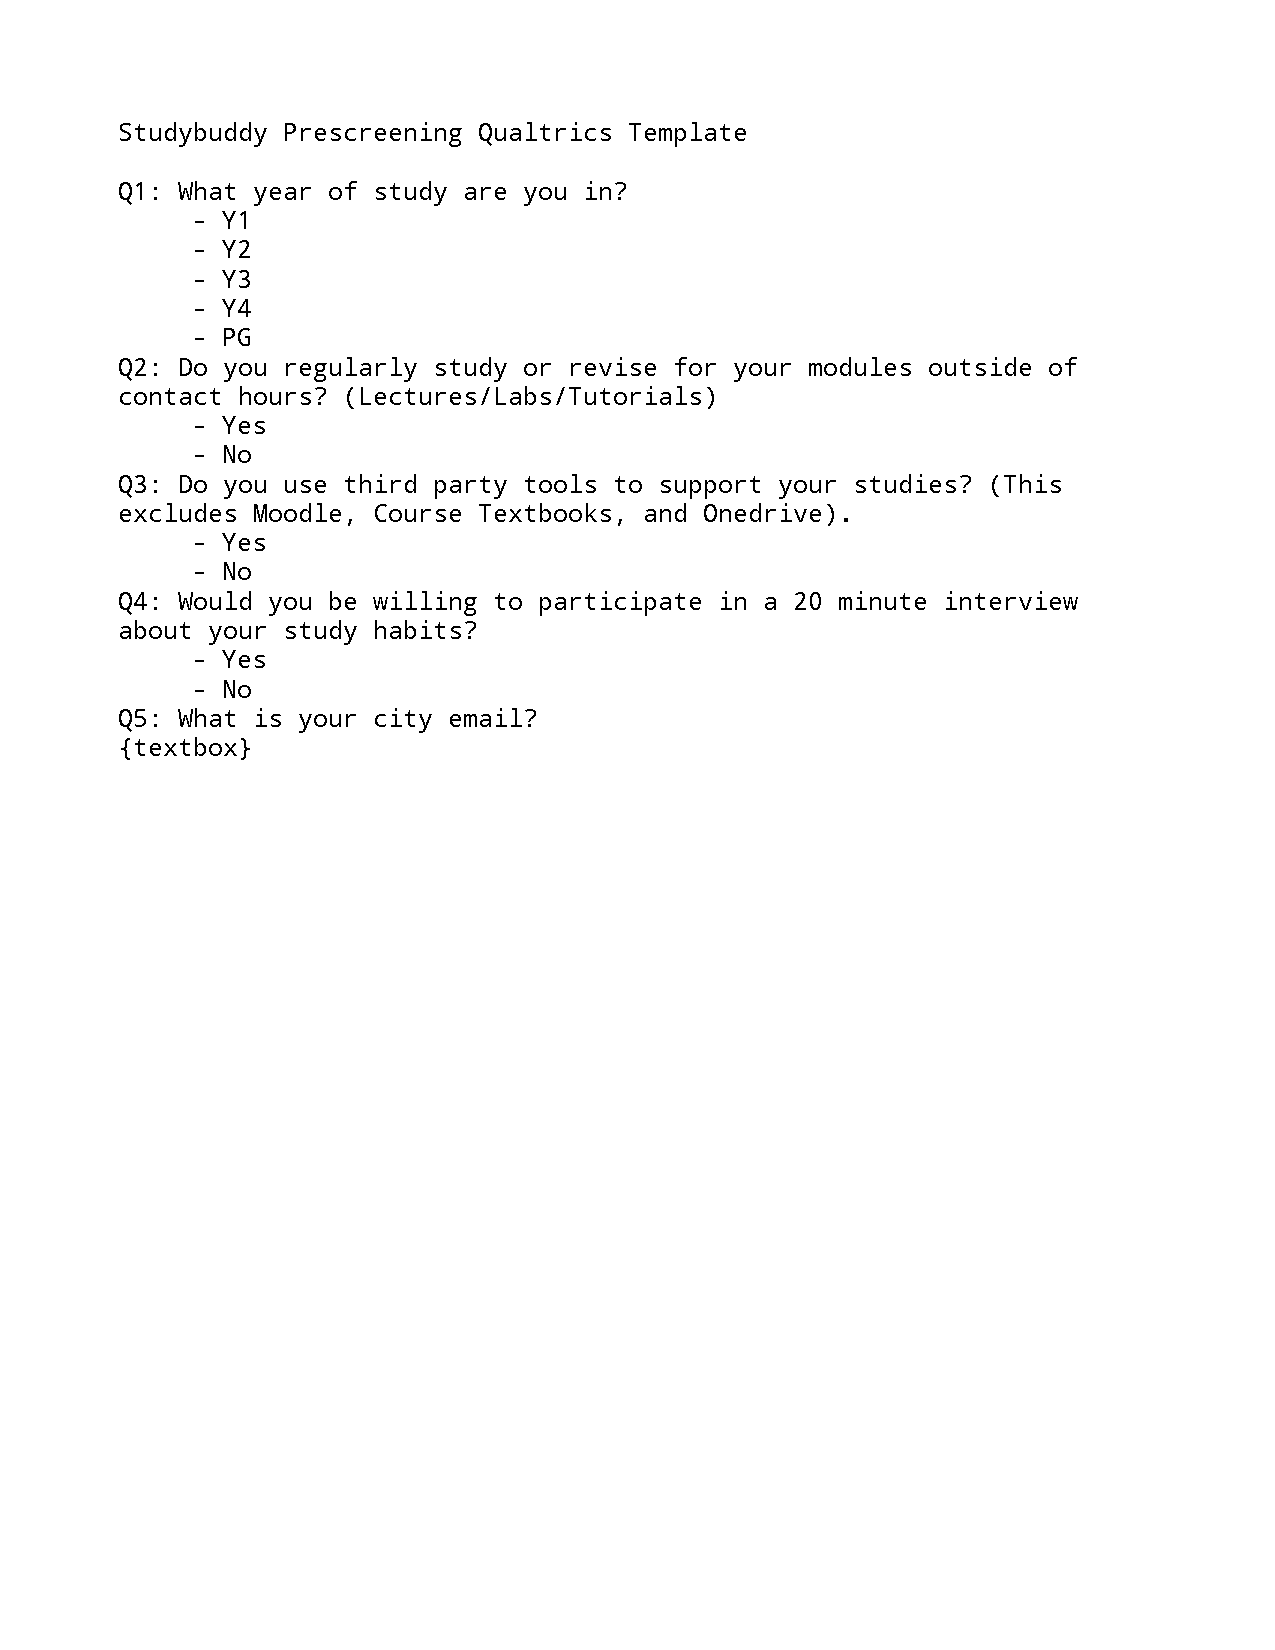
\includepdf[pages=-,pagecommand={\thispagestyle{fancy}}]{../Qualtrics.pdf}

\subsubsection*{Survey responses (anonymised)}

The actual responses exported from Qualtrics, with personally
identifiable columns removed (\texttt{IPAddress},
\texttt{RecipientFirstName} / \texttt{LastName} /
\texttt{Email}, \texttt{ExternalReference},
\texttt{LocationLatitude} / \texttt{Longitude}, and \texttt{Q10} ---
the participant-supplied university email used only to follow up with
qualifying respondents). The full anonymised file is bundled as
\texttt{part-2/qualtricsdata-anonymised.csv}; the tables below
reproduce its content. Ten responses were recorded: two researcher
previews on 2026-03-31 (R1--R2), seven complete real responses
(R3--R7, R9), and two abandoned attempts (R8 at 14\% and R10 at
57\%). Six of the seven complete real responses qualified (Stage~2
or 3, willing to interview, consented to follow-up); the four
interviewed (P1--P4) were drawn from those six.

\paragraph{Question key.} Q1 and Q9 are the consent items; Q5--Q8
are the screener items used against the inclusion criteria in
\S\ref{sec:methodology}.

\begingroup
\setlength{\tabcolsep}{4pt}
\renewcommand{\arraystretch}{1.15}
\begin{longtable}{@{}>{\raggedright\arraybackslash}p{1.0cm}
                    >{\raggedright\arraybackslash}p{14.6cm}@{}}
\toprule
\textbf{Code} & \textbf{Question (verbatim, abridged where indicated)} \\
\midrule
\endhead
Q1 & Consent to participate in the screener (long PIS-style blurb;
     response set: \emph{Acknowledge}). \\
Q5 & ``What year of study are you in?'' (response set: \emph{Stage 1
     / 2 / 3}, where Stage~3 = postgraduate). \\
Q6 & ``Do you study or revise your modules outside of contact hours
     (Lectures/Labs/Tutorials)?'' (\emph{Yes / Sometimes / No}). \\
Q7 & ``Do you use third party tools to support your studies? (This
     excludes Moodle, OneDrive, and course textbooks).'' (\emph{Yes /
     Sometimes / No}). \\
Q8 & ``Would you be willing to participate in a 20 minute interview
     about your study habits?'' (\emph{Yes / No}). \\
Q9 & Consent to providing university email for follow-up
     (\emph{Yes}; blank where the participant did not reach Q9). \\
\bottomrule
\end{longtable}
\endgroup

\paragraph{Responses.} Identifiers \texttt{R1}--\texttt{R10} are
assigned in CSV row order. \emph{Type} is the Qualtrics distribution
channel (\emph{preview} = researcher dry-run; \emph{anon.} = public
survey link, recorded as \texttt{anonymous} in the CSV). \emph{Date}
is the response start date (yyyy-mm-dd); \emph{Dur} is duration in
seconds. Blank cells indicate the respondent abandoned the survey
before reaching that question. The full CSV preserves
\texttt{StartDate}~/~\texttt{EndDate}~/~\texttt{RecordedDate}
timestamps and the original \texttt{ResponseId} per row.

\begingroup
\footnotesize
\setlength{\tabcolsep}{3pt}
\renewcommand{\arraystretch}{1.15}
\begin{longtable}{@{}llllrrlllllc@{}}
\toprule
\textbf{\#} & \textbf{Date} & \textbf{Type} & \textbf{\%} &
\textbf{Dur} & \textbf{Q1} & \textbf{Q5} & \textbf{Q6} &
\textbf{Q7} & \textbf{Q8} & \textbf{Q9} \\
\midrule
\endhead
R1  & 2026-03-31 & preview & 100 & 10  & Acknowledge & Stage 2 & Sometimes & Sometimes & No  &     \\
R2  & 2026-03-31 & preview & 100 & 17  & Acknowledge & Stage 2 & No        & Sometimes & Yes & Yes \\
R3  & 2026-04-02 & anon.   & 100 & 85  & Acknowledge & Stage 2 & Yes       & Sometimes & Yes & Yes \\
R4  & 2026-04-02 & anon.   & 100 & 63  & Acknowledge & Stage 2 & Yes       & Yes       & Yes & Yes \\
R5  & 2026-04-02 & anon.   & 100 & 70  & Acknowledge & Stage 2 & Sometimes & Yes       & Yes & Yes \\
R6  & 2026-04-02 & anon.   & 100 & 46  & Acknowledge & Stage 3 & Sometimes & Sometimes & Yes & Yes \\
R7  & 2026-04-04 & anon.   & 100 & 395 & Acknowledge & Stage 1 & Sometimes & Yes       & Yes & Yes \\
R8  & 2026-03-31 & anon.   &  14 & 72  & Acknowledge &         &           &           &     &     \\
R9  & 2026-03-31 & anon.   &  86 & 153 & Acknowledge & Stage 2 & Sometimes & Yes       & Yes & Yes \\
R10 & 2026-04-06 & anon.   &  57 & 20  & Acknowledge & Stage 2 & Yes       & Yes       &     &     \\
\bottomrule
\end{longtable}
\endgroup

\newpage
\section{Informed Consent Form (Template)}\label{app:consent}
The unsigned ethics-template version of the consent form is reproduced
below. The four signed copies (one per participant) are submitted as
the separate \emph{Signed Informed Consent Forms} PDF (PDF~2), per
the coursework brief's instruction that personally identifiable
information must not appear in the main report.

\includepdf[pages=-,pagecommand={\thispagestyle{fancy}}]{../UCSD-CW-Ethics-Informed Consent Form template-v1.2.pdf}

\newpage
\section{Participant Information Sheet}\label{app:pis}
The Participant Information Sheet provided to all four participants
prior to consent.

\includepdf[pages=-,pagecommand={\thispagestyle{fancy}}]{../UCSD-CW-Ethics-Participant Information Sheet template-v1.2.pdf}

\newpage
\section{Interview Guide (As Used)}\label{app:guide}

Semi-structured guide. Bullets are anchor questions; sub-bullets are
probes used opportunistically. Walkthroughs were elicited at the end
of the substantive content (Block~5) so the participant's verbal
account was not contaminated by the act of demonstration.

\subsubsection*{Block 0. Setup (\textasciitilde2~min)}
\begin{itemize}[leftmargin=1.2em,itemsep=2pt]
    \item Confirm consent form signed; restart recording.
    \item Re-state: anonymised at transcript stage; right to withdraw
          for two weeks; no right or wrong answers.
    \item Brief framing: ``I'm interested in how you actually study,
          not what's recommended. Concrete examples beat generalities.''
\end{itemize}

\subsubsection*{Block 1. Modules \& difficulty (\textasciitilde3~min)}
\begin{itemize}[leftmargin=1.2em,itemsep=2pt]
    \item Walk me through your semester-2 module set.
    \item Which feels hardest right now? Why?
        \begin{itemize}[leftmargin=1em]
            \item Probe: content vs.\ delivery vs.\ assessment vs.\ workload.
            \item Probe for any sub-area within the module that is
                  disproportionately hard.
        \end{itemize}
\end{itemize}

\subsubsection*{Block 2. Daily structure \& prioritisation (\textasciitilde5~min)}
\begin{itemize}[leftmargin=1.2em,itemsep=2pt]
    \item Talk me through a typical study day this semester.
    \item How do you decide what to work on first on any given day?
        \begin{itemize}[leftmargin=1em]
            \item Probe: difficulty, deadline, motivation, mood,
                  external trigger.
            \item Probe horizon: today only, this week, this term?
            \item Probe tracking: how do you know whether you're on
                  track?
        \end{itemize}
    \item Does anything change for exam-style modules vs.\ coursework
          modules?
\end{itemize}

\subsubsection*{Block 3. Resources \& tooling (\textasciitilde5~min)}
\begin{itemize}[leftmargin=1.2em,itemsep=2pt]
    \item What do you actually open when you sit down to revise?
        \begin{itemize}[leftmargin=1em]
            \item Probe Moodle specifically. Friction? What works?
            \item Probe note-taking: where do your notes live?
                  Handwritten, digital, hybrid?
            \item Probe AI: do you use it; for what; what do you not
                  trust it for?
            \item Probe video: YouTube, lecture capture; what for?
        \end{itemize}
    \item When you get stuck on a tutorial question, what do you do
          first, second, third?
\end{itemize}

\subsubsection*{Block 4. Focus, environment, social (\textasciitilde5~min)}
\begin{itemize}[leftmargin=1.2em,itemsep=2pt]
    \item Where do you study? Does location matter?
    \item What breaks your focus? What restores it?
    \item Do you ever study with other people? In what form (in person,
          Discord, study group)? When does that work; when doesn't it?
\end{itemize}

\subsubsection*{Block 5. Walkthrough (\textasciitilde5--10~min)}
\begin{itemize}[leftmargin=1.2em,itemsep=2pt]
    \item Open the device or artefact you actually study with.
          \emph{(For P3, who had no device or artefact present:}
          ``Imagine the exam is in two days; walk me through what you'd
          do, step by step.''\emph{)}
    \item Show me what last night's (or last week's) study session
          looked like, end-to-end.
        \begin{itemize}[leftmargin=1em]
            \item Probe: what was the trigger? what closed it out?
            \item Probe at decision points: ``why did you switch to
                  X?''
        \end{itemize}
\end{itemize}

\subsubsection*{Block 6. Wrap (\textasciitilde2~min)}
\begin{itemize}[leftmargin=1.2em,itemsep=2pt]
    \item Anything I haven't asked about that matters?
    \item Confirm next steps; offer to share findings if interested.
\end{itemize}

\newpage
\section{Full List of Findings}\label{app:findings}

Granular. One observation per row, P-tagged, traced to the theme(s)
in \S\ref{sec:results}. Some findings contribute to multiple themes.

\setlength{\emergencystretch}{3em}
\begin{longtable}{@{}>{\raggedright\arraybackslash}p{0.8cm}>{\raggedright\arraybackslash}p{10.4cm}>{\raggedright\arraybackslash}p{2.6cm}>{\raggedright\arraybackslash}p{1.5cm}@{}}
\toprule
\textbf{\#} & \textbf{Finding} & \textbf{P} & \textbf{Theme} \\
\midrule
\endhead
F1  & Mechatronics ranked hardest by 3 of 4 participants; reason given is theoretical/applied content (control systems, ODEs, physics formulas). & P1, P2, P4 & T1 \\
F2  & The cognitive bottleneck is \emph{which} equation to apply, not arithmetic. & P1, P2, P3 & T1 \\
F3  & Tutorial sheets are the central revision artefact across all participants. & P1, P2, P3, P4 & T1, T2 \\
F4  & Provided Moodle solutions often give a numerical answer with no working. & P1 & T1, T5 \\
F5  & Tutorial answers are sometimes uploaded ${\sim}1$~week after the tutorial, breaking the catch-up loop for missed sessions. & P4 & T1, T5 \\
F6  & Past papers / mocks \textbf{with worked solutions} are the most-wanted missing resource. & P3, P4 & T1, T5 \\
F7  & Worked examples are valued as a \emph{thought-process model}, not just answer-checking. & P4 & T1 \\
F8  & Mock papers are used as a diagnostic to guide subsequent revision allocation. & P3, P4 & T1, T2 \\
F9  & When stuck, students cascade through nearest-similar-tutorial $\rightarrow$ AI $\rightarrow$ YouTube $\rightarrow$ pre-exam peer help. & P3, P4 & T1, T4 \\
F10 & All four participants use AI to fill explanation/procedure gaps; none uses it as a primary workflow. & P1, P2, P3, P4 & T1 \\
F11 & AI hallucination of \emph{working} (correct answer, wrong steps) is an explicit fear. & P2 & T1 \\
F12 & AI is treated as a last resort by some, with deliberate exhaustion of other sources first. & P4 & T1 \\
F13 & NotebookLM (or equivalent dedicated study-AI tool) is known and used by only 1 of 4; the other 3 have not encountered it. & P1 (used); P2, P3, P4 (not) & T1, T5 \\
F14 & NotebookLM use is exam-time-only, not term-time. & P1 & T1 \\
F15 & NotebookLM was discovered accidentally while looking for a Notion alternative. & P1 & T5 \\
F16 & YouTube is used for \emph{topic understanding}, not problem-solving. & P2, P3, P4 & T1 \\
F17 & YouTube is also a known rabbit-hole risk (``educational\dots\ at the end it's really nothing''). & P2 & T3 \\
F18 & Each participant's prioritisation rule differs: difficulty (P1), session-count goal (P2), deadline (P3), motivation (P4). & P1, P2, P3, P4 & T2 \\
F19 & Strategy varies by module \emph{type} (coursework vs.\ exam-based) for P4. & P4 & T2 \\
F20 & Coursework-only modules receive little or no formal revision effort. & P1 & T2 \\
F21 & No participant plans more than ${\sim}3$~days ahead. & P1, P2, P3, P4 & T2 \\
F22 & No participant tracks progress with anything beyond mental goals. & P2, P3, P4 & T2 \\
F23 & Effort, not output, is the implicit success metric for daily study. & P2 & T2 \\
F24 & A \textbf{last-session refresher} ritual is used as a session-start re-entry pattern. & P4 & T2 \\
F25 & Some participants \textbf{read ahead} by topic before lectures, using Google $\rightarrow$ YouTube. & P4 & T2 \\
F26 & Time-of-day preferences are mutually incompatible across the cohort: 20--23h (P1), 14--16h (P2), 22--24h (P3), timetable-gap (P4). & P1, P2, P3, P4 & T2, T3 \\
F27 & A decompression / ``studying mindset'' ritual is required before serious work begins. & P1 & T3 \\
F28 & Movement (people moving in shared rooms) is cited as the dominant non-noise distraction. & P1 & T3 \\
F29 & Phone checking is reported as habitual / non-volitional. & P2 & T3 \\
F30 & Same-machine gaming/study creates a context-switch trap, mitigated by physical re-priming (moving keyboard). & P2 & T3 \\
F31 & Some students leave home for serious coursework because the bedroom is associated with leisure. & P4 & T3 \\
F32 & Multi-monitor / side-by-side material display is a focus enabler for some. & P2, P4 & T3 \\
F33 & Single-earbud listening is used as an ambient focus signal. & P1 & T3 \\
F34 & Long commute to campus is a deterrent to using campus study spaces. & P2 & T3 \\
F35 & Family activity is mitigated through unspoken cues (P1), late-night study (P3), or time-shifting (P4 weekday daytime when family is out). & P1, P3, P4 & T3 \\
F36 & Pre-exam group study via Discord (or in-person) is used by all four participants. & P1, P2, P3, P4 & T4 \\
F37 & Coordination of pre-exam group study is spontaneous (``@everyone'', ``who wants to join?'') with no scheduling. & P1, P3, P4 & T4 \\
F38 & Group sessions are vulnerable to off-topic chatter and pace mismatch. & P1, P3 & T4 \\
F39 & Group sessions also have specific value: screen-shared question solving and explain-to-learn. & P4 (explain-to-learn); all four (screen-share) & T4 \\
F40 & Group projects are typically led via task delegation rather than collaborative working. & P1, P2 & T4 \\
F41 & All four participants treat Moodle as the inescapable on-ramp to course material. & P1, P2, P3, P4 & T5 \\
F42 & Moodle UI friction (clicks, navigation overhead) is explicitly cited. & P2 & T5 \\
F43 & Lecturer-by-lecturer inconsistency in Moodle layout forces re-orientation cost per module. & P2 & T5 \\
F44 & Monolithic uploads (single 300-page PowerPoint) are intimidating and discourage engagement. & P2 & T5 \\
F45 & Drip-release of lecture material prevents look-ahead planning. & P4 & T5 \\
F46 & Each participant builds a personal external memory beside Moodle: Notion (P1), handwritten colour-coded notes + formula corkboard (P2), iPad folder hierarchy (P4); P3 downloads ad-hoc. & P1, P2, P3, P4 & T5 \\
F47 & Spatial / ambient cues (the wall-mounted formula corkboard) act as passive retrieval prompts. & P2 & T5 \\
F48 & Lab sessions can be a learning blocker for non-content reasons (faulty hardware, weak TA support). & P4 & (out-of-scope for design) \\
F49 & Lecture capture is only useful when the camera shows the whiteboard. & P1 & (out-of-scope for design) \\
\bottomrule
\end{longtable}

\subsubsection*{Key Requirements (full descriptions)}\label{app:requirements}

The summary in \S\ref{sec:results} lists R1--R10 as headlines; the full
descriptions and the underlying findings each requirement traces to are
below. Square-bracket tags read as \texttt{[Theme(s); Finding(s)]}.

\begin{itemize}[leftmargin=2.4em,itemsep=2pt]
  \item[\textbf{R1}] Surface tomorrow's class card on the home screen
        as the trigger artefact (module, slot, room, sources count).
        [T1, T2; F3, F18, F26]
  \item[\textbf{R2}] Provide a one-paragraph recap of the last
        session built from the connected sources, with bolded terms
        deep-linked back into the underlying slide ranges. [T1; F2, F24]
  \item[\textbf{R3}] Show step-by-step worked solutions with
        clear source attribution before any AI-generated text;
        directly address the fear of AI getting the working wrong.
        [T1; F4, F11]
  \item[\textbf{R4}] Treat past papers and mocks as a first-class
        source for the same worked-solution flow, not a separate
        feature. [T1; F6, F8]
  \item[\textbf{R5}] Connect to and coexist with the student's
        existing external memory: Moodle, MyTimetable and a notes
        provider (Notion / iPad / Drive). Do not replace.
        [T5; F41, F46]
  \item[\textbf{R6}] Accept a paper or file capture (snap a tutorial
        sheet, open a downloaded PDF) into the worked-solution
        flow. [T1; F3, F46]
  \item[\textbf{R7}] Work inside an informal, deadline-driven
        rhythm: no streaks, badges, or long-horizon planning.
        [T2; F21, F22]
  \item[\textbf{R8}] Plan rows must show \emph{what}, \emph{why this
        size}, and \emph{when due}; the ``why'' is the bit students
        cannot get from any current tool. [T2; F18--F20]
  \item[\textbf{R9}] Adapt to the student's own prioritisation rule
        (difficulty, deadline, session-count, motivation) rather
        than imposing a single ranking. [T2; F18]
  \item[\textbf{R10}] Capture felt-readiness per topic at session
        wrap-up and feed it forward into tomorrow's briefing,
        mirroring P4's last-session refresher ritual.
        [T2; F23, F24]
\end{itemize}

\newpage
\section{Interview Summaries}\label{app:summaries}

One paragraph per participant, drawn from the cleaned transcripts.
Quotes are referenced as \texttt{[Px Iy:zz]} where \texttt{Iy} is the
interview file (\texttt{Interview1.md}--\texttt{Interview4.md}) and
\texttt{zz} is the line number in the cleaned markdown.

\subsubsection*{P1}
Studies in a fixed \textbf{20:00--23:00 evening block} after commuting
home, eating, and ``decluttering my mind'' [P1~I1:181--185]. Pre-reads
slides when uploaded the night before; otherwise reviews the day's
content. Prioritises within a day by difficulty [P1~I1:85]; across exams
by exam order [P1~I1:93]. Bedroom for focus work; living room for
low-stakes content (pneumatic / hydraulic systems); campus silent-study
room between classes [P1~I1:161]. Most distracted by \textbf{movement}
rather than sound, mitigated by a single earbud
[P1~I1:137,~153]. Tools: Moodle as gateway; \textbf{Notion} for note
storage; \textbf{NotebookLM} for \textbf{exam-time quiz generation}
(``I don't make flashcards: I plug them into NotebookLM''
[P1~I1:291]). Lecture capture as a reactive fallback, but its usefulness
depends on whether the camera shows the board [P1~I1:347]. Group study
limited to ad-hoc \textbf{pre-exam Discord calls} with screen-shared
question solving; attends few because off-topic chatter and slow pace
put them off [P1~I1:201--209]. Key pain point: tutorial solutions on
Moodle give numerical answers without working (``560 kg for mass''
[P1~I1:263]).

\subsubsection*{P2}
Same modules. Studies \textbf{post-lunch (14:00--16:00)};
\textbf{refuses evening study} (``after four\dots\ I refuse to work''
[P2~I2:109]). Sets mental daily goals of N ``sessions'' with no formal
tracking [P2~I2:277--281]. Same gaming PC for play and study; treats
this as the dominant focus trap and counters it physically by
\textbf{moving the keyboard aside} when studying [P2~I2:233]. Father
permanently in living room, so the desk is the only available space;
campus not viable due to a 40--50~min commute
[P2~I2:181,~189]. \textbf{Heavy hand-writing practice} with an explicit
colour scheme (blue body, red highlights, pencil footnotes
[P2~I2:329]) and a \textbf{wall-mounted formula corkboard} next to their PC,
used as an ambient retrieval cue every time they pass
[P2~I2:133]. Two-monitor setup (lecture~|~tutorial) with a YouTube tab
for music [P2~I2:315]. AI used to fill in \textbf{procedure} the slides
skip, with explicit \textbf{hallucination fear}: ``I'm scared of AI
getting the calculation totally wrong: showing you the right result,
but not the right way to get there'' [P2~I2:169]. Has not heard of
NotebookLM [P2~I2:141]. Phone-checking is habitual / non-volitional
[P2~I2:217]. Walks with their mum reset focus [P2~I2:347--355].

\subsubsection*{P3}
Same modules. Day is \textbf{mostly unstructured}; only project
deadlines or upcoming exams force structure [P3~I3:69]. Studies
\textbf{late-night, ${\sim}22$:00--24:00}, specifically to dodge family
activity [P3~I3:241]. Bedroom + computer; doesn't study at uni at all
[P3~I3:173]. Quiet + clean + tidy is the precondition
[P3~I3:177--189]. Tools: Moodle (tutorial sheets + lecture notes), AI
for missing worked examples, YouTube for understanding (``Indian guy
who's just got it on'' [P3~I3:125]). Cynical about AI (``AI all the way
down'' [P3~I3:165]). No NotebookLM, no Notion, no flashcards
[P3~I3:129--133]. Strategy: deadline-based exam priority; \textbf{mock
papers as diagnostic} (do a mock first, scale revision to gap)
[P3~I3:97--101]. Wants past papers with worked solutions
[P3~I3:161]. Mostly works alone; pre-exam Discord calls when nearer to
exams [P3~I3:265] but distracted by people who ``just talk to me''
[P3~I3:257].

\subsubsection*{P4}
Same modules. Ranks mechatronics hardest for \textbf{non-content
reasons}: faulty Arduino kits, unhelpful TAs, ``running around in
circles'' [P4~I4:47--55]. No clock-based daily structure; uses
\textbf{timetable gaps} (free Wednesday this term) and reading week as
study days [P4~I4:115--119]. Prioritises by \textbf{motivation}
(``directly correlated'' with effort) [P4~I4:123--127]. Strategy varies
by module type: \textbf{coursework} = hands-on project work;
\textbf{exam} = past papers + tutorial pass [P4~I4:139].
\textbf{Multi-monitor mandatory}: content open beside questions
[P4~I4:189--197]. Bedroom for exams, but \textbf{leaves home for
coursework} because the bedroom is associated with leisure (``removing
myself from that at university'' [P4~I4:233]). Smart tablet (iPad) for
notes, with a \textbf{subject $\rightarrow$ exam $\rightarrow$ topic
folder hierarchy} [P4~I4:255]. \textbf{Last-session refresher} ritual:
re-reads previous session's notes on the second monitor before starting
the next session [P4~I4:259]. \textbf{Reads ahead} by topic before
lectures, using Google $\rightarrow$ YouTube to build prior context
[P4~I4:91,~107]. YouTube is for \emph{topic understanding}, not
problem-solving [P4~I4:325]. AI is \textbf{last-resort} when stuck after
pattern-matching to a similar tutorial [P4~I4:313]. Moodle pain: hates
\textbf{drip-release} (wants the whole semester upfront to plan ahead)
and \textbf{delayed tutorial answers} [P4~I4:103,~159--163]. Group
study is \textbf{deadline-driven panic sessions}, used to
\textbf{explain topics to others} as a learning device [P4~I4:247].

\newpage
\section{Evidence of Analysis}\label{app:analysis}

\subsubsection*{Approach}
Analysis followed \textcite{braun2006}'s six-phase reflexive thematic
analysis: (1)~familiarisation with cleaned transcripts; (2)~line-level
open coding (\S\ref{app:analysis-coding} below, sample of
\textbf{P2}); (3)~clustering of codes into candidate groups
($\alpha$--$\varepsilon$, \S\ref{app:analysis-clusters}) in a digital
affinity diagram (\S\ref{app:analysis-figjam}); (4)~theme review
against the source extracts; (5)~final theme definition (T1--T5,
reported in \S\ref{sec:results}).

\subsubsection*{Phase 3. Digital affinity diagram (FigJam)}
\label{app:analysis-figjam}

Open codes were clustered in FigJam to produce a clean, labelled
affinity diagram. The five emergent groups
(A-E) map directly onto T1--T5
(\S\ref{sec:results}); a sixth ``Did not cluster'' column captures
extracts kept for transparency, per Braun \& Clarke's guidance that
not every data extract has to feed a theme.

\includepdf[pages=-,pagecommand={\thispagestyle{fancy}}]{figjam.pdf}

\subsubsection*{Phase 2. Open codebook (sample: P2)}
\label{app:analysis-coding}

A representative slice of the line-level open coding for P2. The full
codebook for P1--P4 lives in the working analysis document
(\texttt{part-2/analysis.md}~\S3); the sample below shows the level of
granularity used and the line-traceable mapping from raw extract to
descriptive code label.

\setlength{\emergencystretch}{3em}
\begin{longtable}{@{}>{\raggedright\arraybackslash}p{1.0cm}>{\raggedright\arraybackslash}p{8.4cm}>{\raggedright\arraybackslash}p{6.0cm}@{}}
\toprule
\textbf{Line} & \textbf{Quote (excerpt)} & \textbf{Code} \\
\midrule
\endhead
77      & ``Which equation to use\dots\ in maths, they just give you the formulas. The physics ones, you need to think it through, take the formula and change it completely.'' & equation selection is the bottleneck \\
109     & ``After four, in the evening, I refuse to work.'' & refuses evening study \\
133     & ``Every time I pass, I can just read this and keep getting the context back.'' & corkboard as ambient retrieval cue \\
137     & ``Different colours\dots\ physics-new\dots\ physics\dots\ put it together.'' & colour-coded topic separation \\
145     & ``We have so many clicks\dots\ the lecturers don't organise it the same way\dots\ the whole lecture in one PowerPoint, 300 pages long, you just get intimidated.'' & Moodle: click friction; lecturer inconsistency; monolithic-upload intimidation \\
161     & ``I had to use AI to explain how to find it.'' & AI as procedure explainer \\
169     & ``AI getting the calculation totally wrong: showing you the right result, but not the right way to get there.'' & AI hallucinated-working fear \\
205     & ``I'll take my keyboard and put it on the side.'' & keyboard relocation as gaming dis-prime \\
277     & ``I'm just keeping it in my mind'' (goals). & mental-only daily goals \\
281     & ``I'm going to do sessions 1, 2 and 3.'' & session-count daily goals \\
285     & ``If it was tough and I worked a lot, I will say `okay, that's fine for today'.'' & effort, not output, as success \\
311     & ``I'll try to find a solution inside the lecture notes, which never happens.'' & lecture-doesn't-have-solution gap \\
315     & ``Two screens\dots\ project the lecture on one screen and the tutorial on the other.'' & two-monitor split (lecture~/~tutorial) \\
329     & ``Blue, the red is just to highlight very important stuff, and pencil are full note notes.'' & handwritten colour scheme \\
347     & ``She just proposes to me to go out for like half an hour, an hour to go and walk\dots\ brings me back down.'' & walk break resets focus \\
\bottomrule
\end{longtable}

\subsubsection*{Phase 3. Code-cluster $\rightarrow$ theme map}
\label{app:analysis-clusters}

\begin{itemize}[leftmargin=1.2em,itemsep=4pt]
    \item \textbf{Cluster a:} equation selection and worked
          examples; AI procedure-explainer + hallucination fear;
          tutorial $\rightarrow$ AI $\rightarrow$ YouTube
          $\rightarrow$ peer cascade.
          \\\emph{Feeds} \textbf{T1:} ``Which equation?''
    \item \textbf{Cluster b:} prioritisation rule (one per
          participant); time-of-day windows; horizon ${\leq}3$~days;
          mental-only goals; effort-as-success.
          \\\emph{Feeds} \textbf{T2:} prioritisation is personal and
          rarely tracked.
    \item \textbf{Cluster c:} spatial / temporal / physical
          focus levers (room choice, single earbud, keyboard
          relocation, multi-monitor, leaving home for coursework).
          \\\emph{Feeds} \textbf{T3:} focus is engineered, not willed.
    \item \textbf{Cluster d:} pre-exam Discord; spontaneous
          coordination; off-topic and pace-mismatch failure modes;
          screen-share and explain-to-learn value.
          \\\emph{Feeds} \textbf{T4:} group study is exam-shaped,
          ad-hoc, brittle.
    \item \textbf{Cluster e:} Notion, NotebookLM,
          handwritten plus corkboard, iPad folder hierarchy, ad-hoc
          download; Moodle friction (clicks, lecturer inconsistency,
          drip-release, monolithic uploads).
          \\\emph{Feeds} \textbf{T5:} Moodle is a delivery channel;
          everyone builds a personal external memory beside it.
    \item \textbf{Did not cluster:} snacking patterns; lecture
          capture board-visibility; lab failure cycle; off-syllabus
          drift. Kept for transparency.
\end{itemize}

\newpage
\section{Walkthrough / Observation Notes}\label{app:observation}

Behavioural notes only; interpretation is in \S\ref{sec:results} and
the analysis appendix above. The CW2 brief requires walkthroughs in at
least two interviews; all four carried one. P1, P2 and P4 are
observation-rich (live screen-share or physical artefacts); P3 gave a
brief verbal scenario walkthrough only and is included for completeness
in \S\ref{app:obs-p3}.

\subsubsection*{P1: live screen-share}\label{app:obs-p1}
\begin{itemize}[leftmargin=1.2em,itemsep=2pt]
    \item \textbf{Setting.} P1's actual home setup; bedroom desk;
          framed explicitly as ``my actual setup, which I have at
          home'' [P1~I1:243]. Time of demonstration: afternoon, but
          the demonstrated workflow is the 20:00--23:00 evening block.
    \item \textbf{Sequence (Moodle).} Opened Moodle. Navigated to a
          mechatronics tutorial sheet. Stated the typical pattern:
          \textbf{attempt the tutorial question first}, then ``as soon
          as I don't understand something, I'll just download the
          solutions'' [P1~I1:255]. Showed the solutions file: a
          \textbf{numerical-only} ``560 kg for mass'' with no working
          [P1~I1:263]. Visible irritation. Noted that worked solutions
          are released \emph{after} the tutorial session [P1~I1:267].
    \item \textbf{Sequence (NotebookLM).} Switched to NotebookLM.
          Showed an \textbf{existing} notebook with a ``BJT quiz'' and
          pre-loaded source nodes [P1~I1:295]. Re-ran the
          upload-and-quiz flow live: navigated to local files, opened
          a probability-notes PDF (Bayes' theorem content), uploaded
          it, generated a quiz, set the difficulty
          [P1~I1:303--311]. Friction: low.
    \item \textbf{Tools visible on screen.} Moodle (browser), file
          system (file picker), NotebookLM (browser). Notion was
          referenced but not opened.
    \item \textbf{Key moments.} Fast switch from Moodle to NotebookLM:
          tools are kept separate by purpose. ``I bumped into
          [NotebookLM] by accident\dots\ looking for the best
          alternative to Notion'' [P1~I1:307]. Confirmed exam-time-only
          use [P1~I1:329].
    \item \textbf{What was not observed.} No demonstration of the
          lecture-capture fallback, Notion, or a Discord study call
          (described verbally only).
\end{itemize}

\subsubsection*{P2: physical artefacts}\label{app:obs-p2}
\begin{itemize}[leftmargin=1.2em,itemsep=2pt]
    \item \textbf{Setting.} P2 did \emph{not} screen-share: laptop was
          not present in the interview room. Walkthrough was conducted
          by demonstrating physical artefacts to the camera, plus
          verbal reconstruction.
    \item \textbf{Artefact 1, formula corkboard.} P2 panned the
          camera to show their room: globe, PC, and a wall-mounted
          \textbf{corkboard} with hand-written formula notes pinned
          next to the desk [P2~I2:133]. Pointed out
          \textbf{colour-coded columns} for different topic areas
          [P2~I2:137]. Stated the corkboard is used as an
          \textbf{ambient retrieval cue}: ``every time I pass, I can
          just read this and keep getting the context back''
          [P2~I2:133]. Photographs of the artefact are reproduced in
          Figures~\ref{fig:p2-cork1}--\ref{fig:p2-cork3}.
    \item \textbf{Artefact 2, handwritten tutorial sheet on
          eigenvalues / determinants.} Showed an example sheet
          [P2~I2:329]. Colour scheme observed:
          \textbf{Blue}~--~body text / standard working;
          \textbf{Red}~--~highlighted important content;
          \textbf{Pencil}~--~footnotes / less-important annotations.
          Content had been copied from a YouTube tutorial onto the
          sheet by hand.
    \item \textbf{Verbal walkthrough, typical session.}
          Two-monitor split (lecture / tutorial) [P2~I2:315]; YouTube
          tab open for music [P2~I2:315]; tries to find the connection
          between lecture content and tutorial questions
          [P2~I2:303--311]; AI invoked when the lecture skips
          procedure [P2~I2:311]; Khan-Academy-style tutor videos for
          explanation, top result usually accepted [P2~I2:319--323].
    \item \textbf{Physical re-priming behaviour.} Keyboard moved to
          the side to break gaming-context association
          [P2~I2:205,~233]. Bed behind chair as overflow surface for
          papers [P2~I2:197--203].
    \item \textbf{Distractions described in situ.} Reflexive
          phone-check (``two or three times, it's just a habit''
          [P2~I2:217]); not notification-driven. Walks with mum used
          as a focus reset [P2~I2:347--355].
    \item \textbf{What was not observed.} No live screen interaction;
          no Moodle navigation; no AI tool open during the interview.
\end{itemize}

\begin{figure}[ht]
\centering
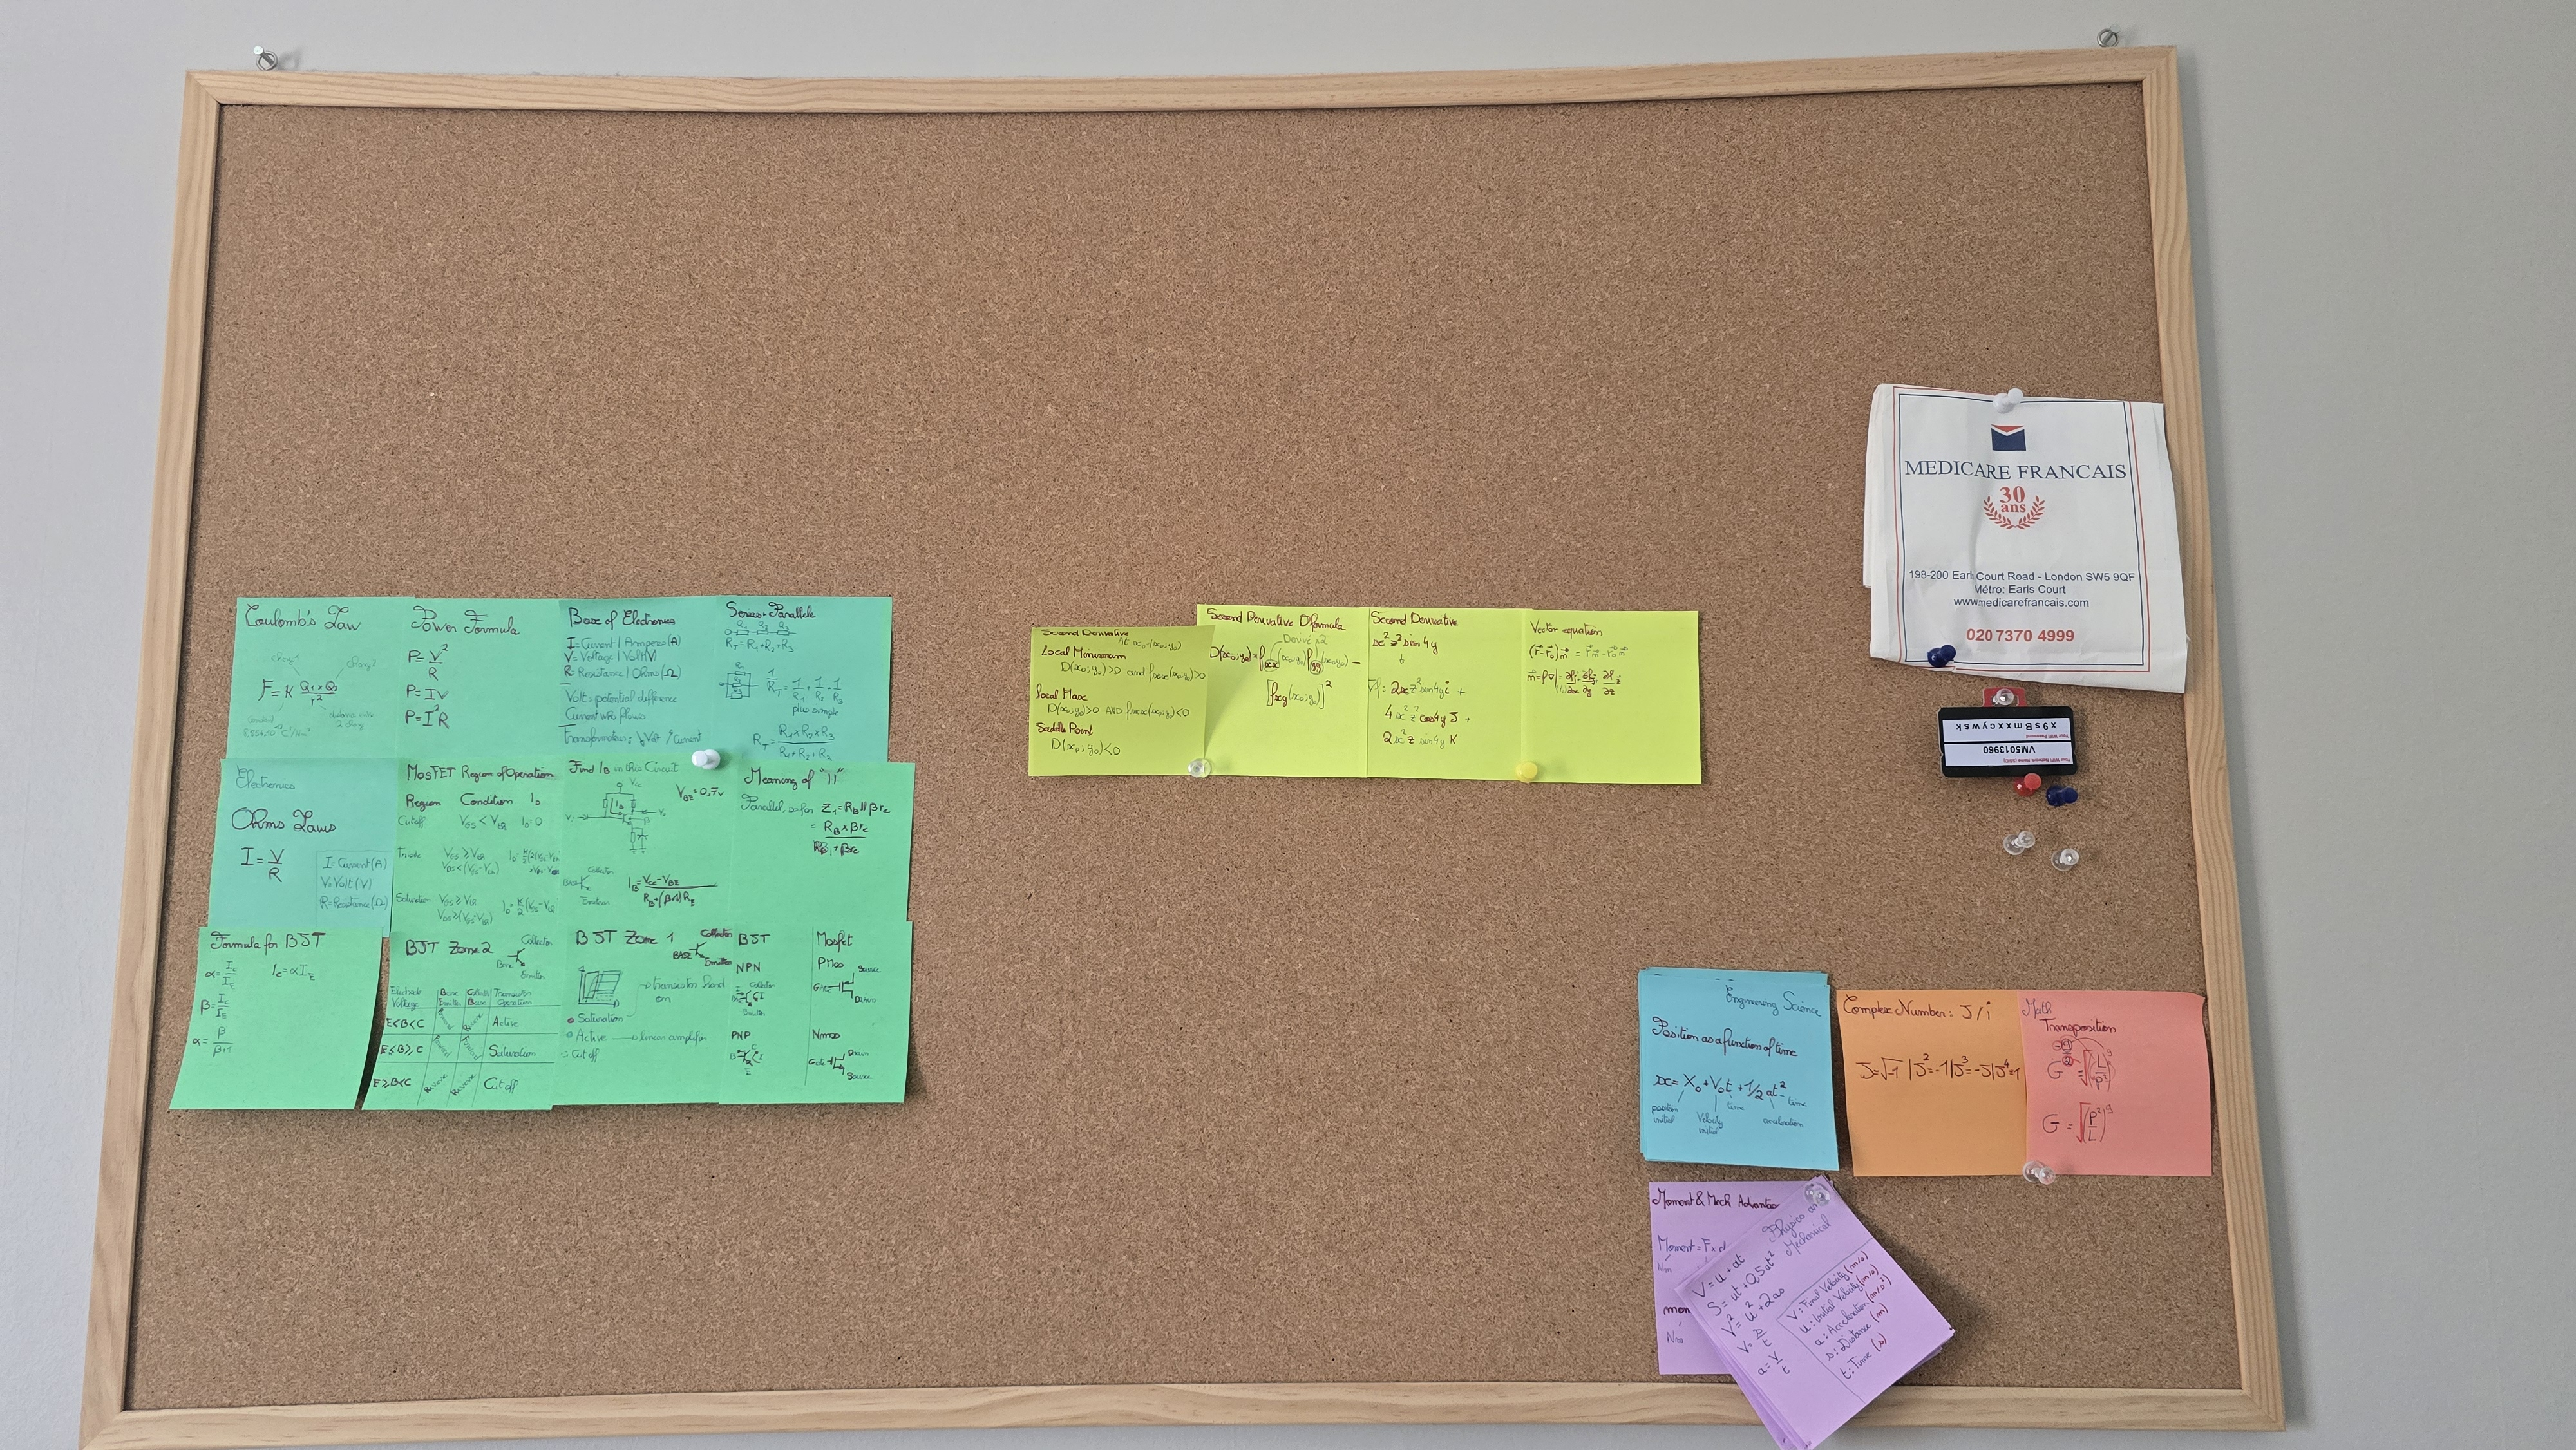
\includegraphics[width=0.78\linewidth]{Pictures of Cork Board/1000299771.jpg}
\caption{P2's wall-mounted formula corkboard, photographed during the
interview. Hand-written formula notes pinned in colour-coded columns,
positioned next to P2's desk for ambient retrieval [P2~I2:133].}\label{fig:p2-cork1}
\end{figure}

\begin{figure}[ht]
\centering
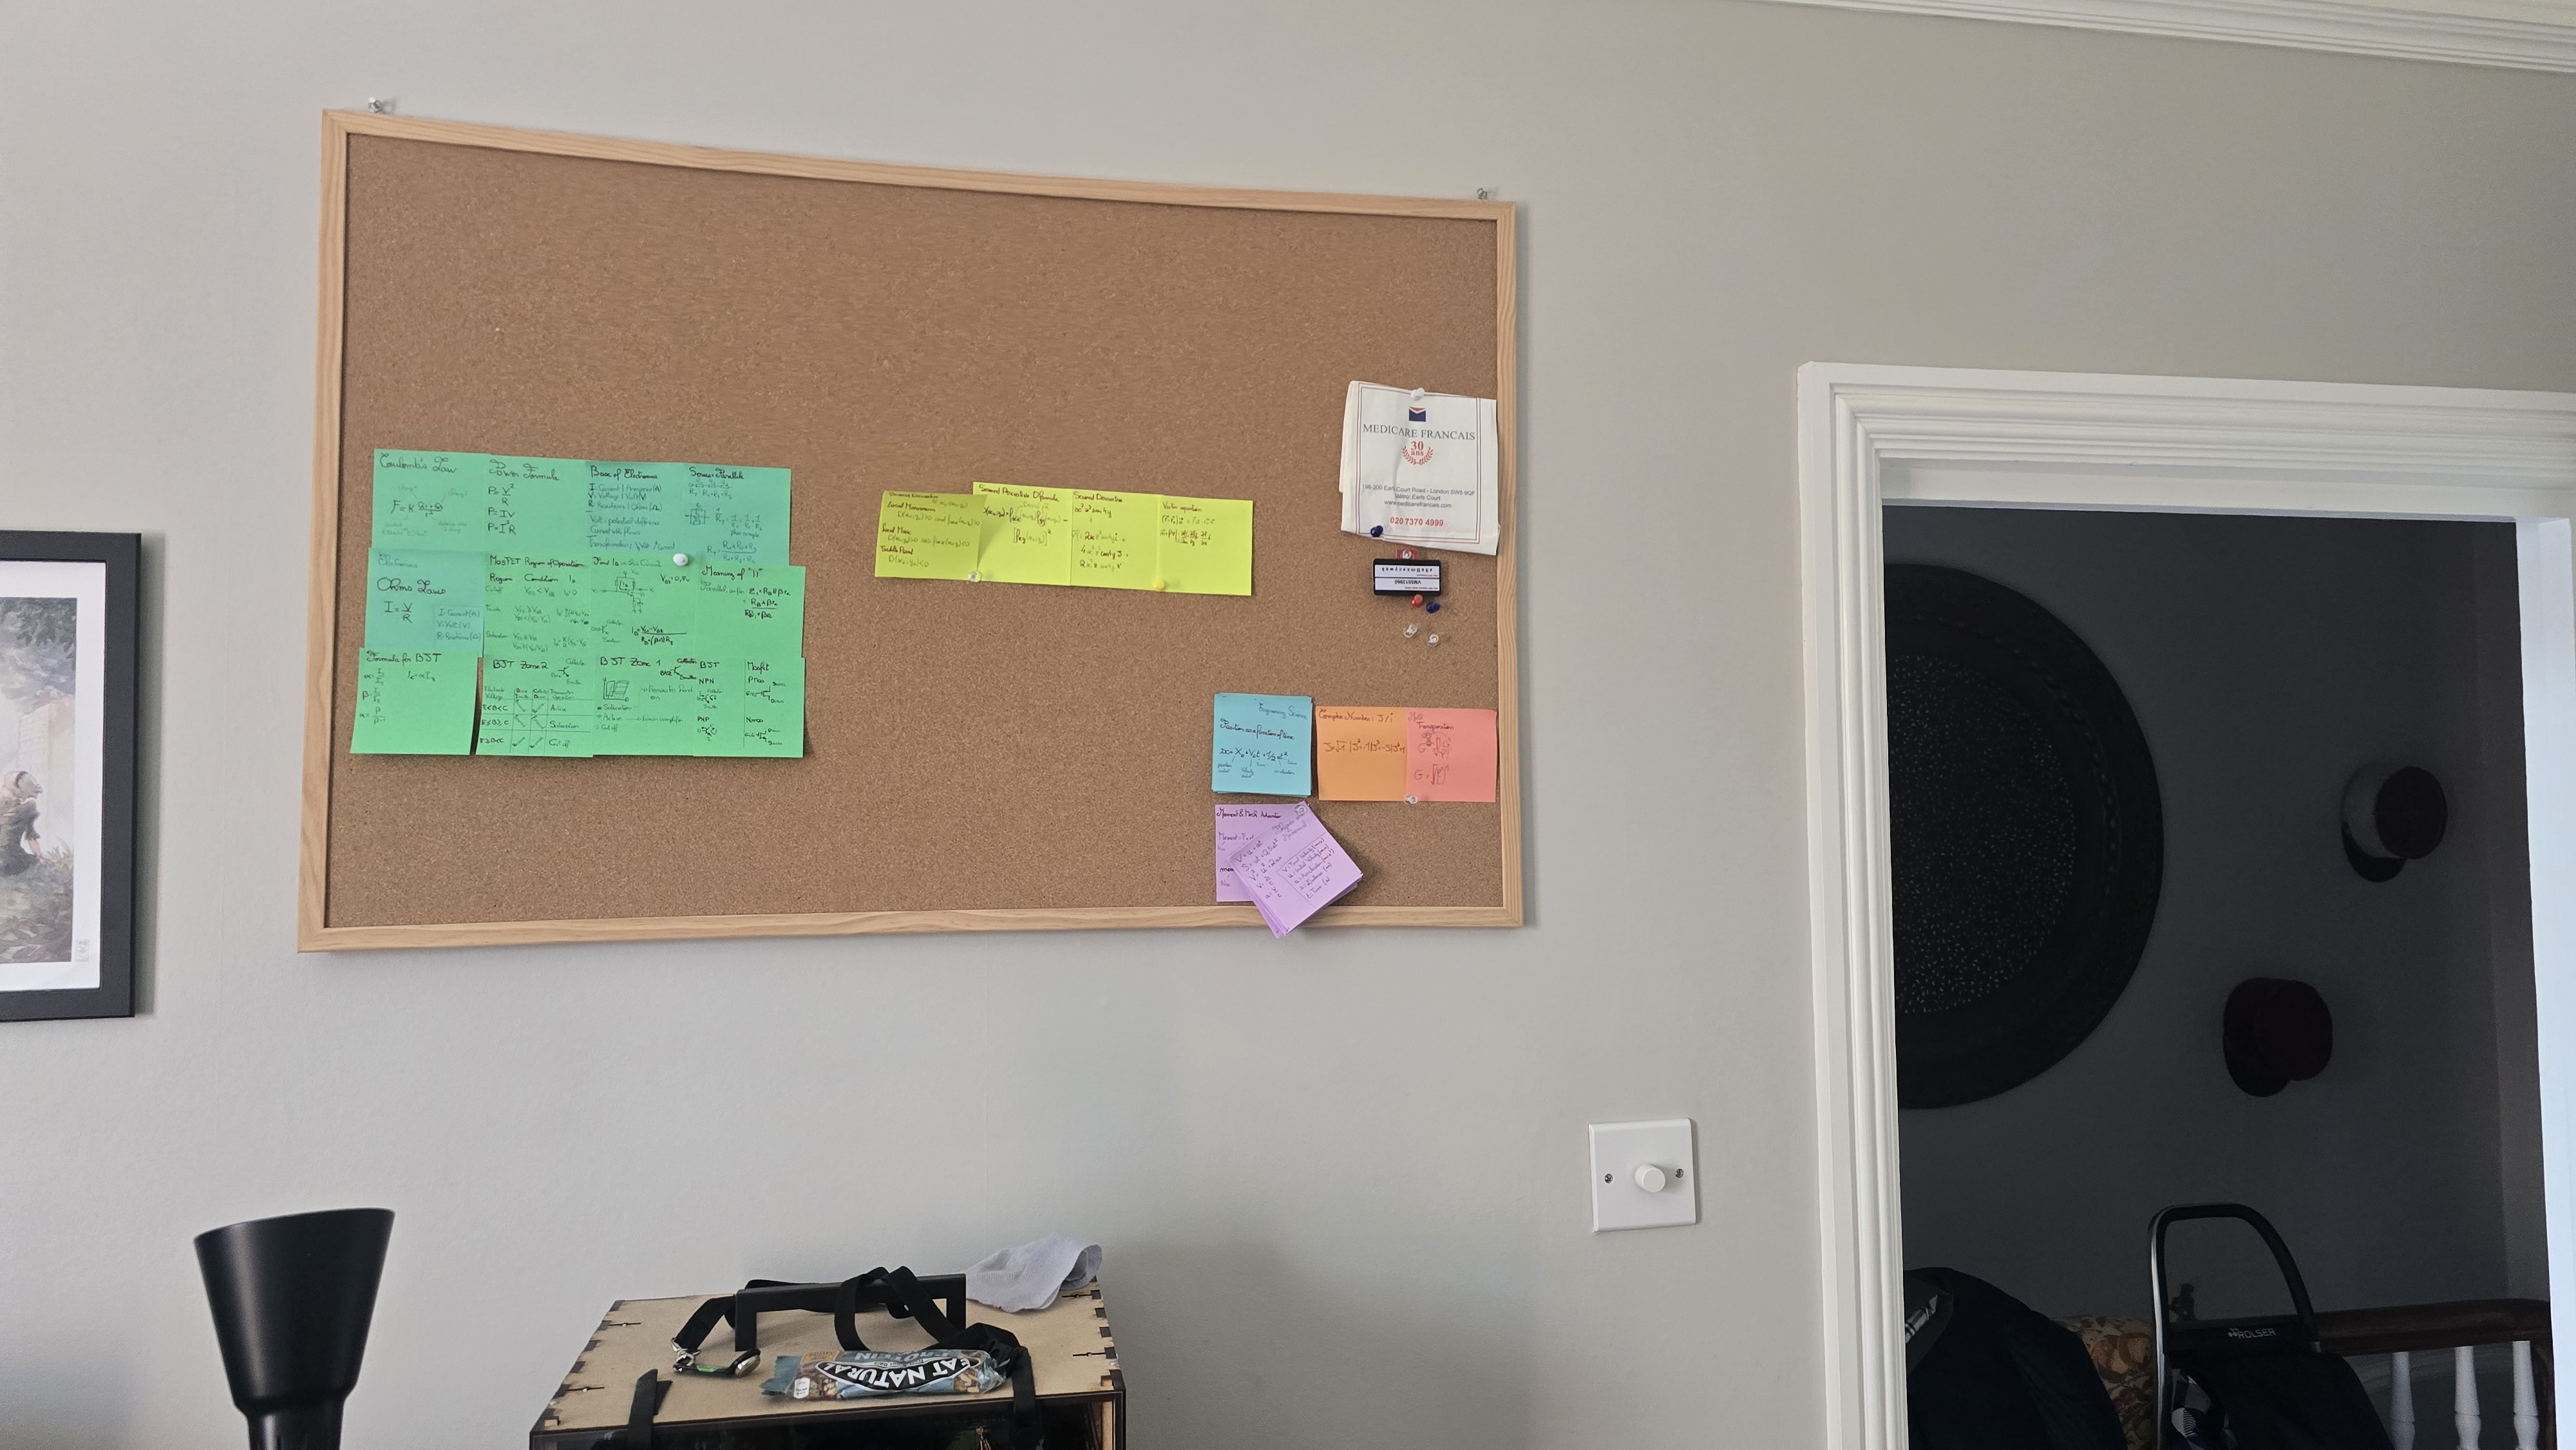
\includegraphics[width=0.78\linewidth]{Pictures of Cork Board/1000299772.jpg}
\caption{Detail of P2's corkboard showing the colour-coded grouping
P2 described [P2~I2:137].}\label{fig:p2-cork2}
\end{figure}

\begin{figure}[ht]
\centering
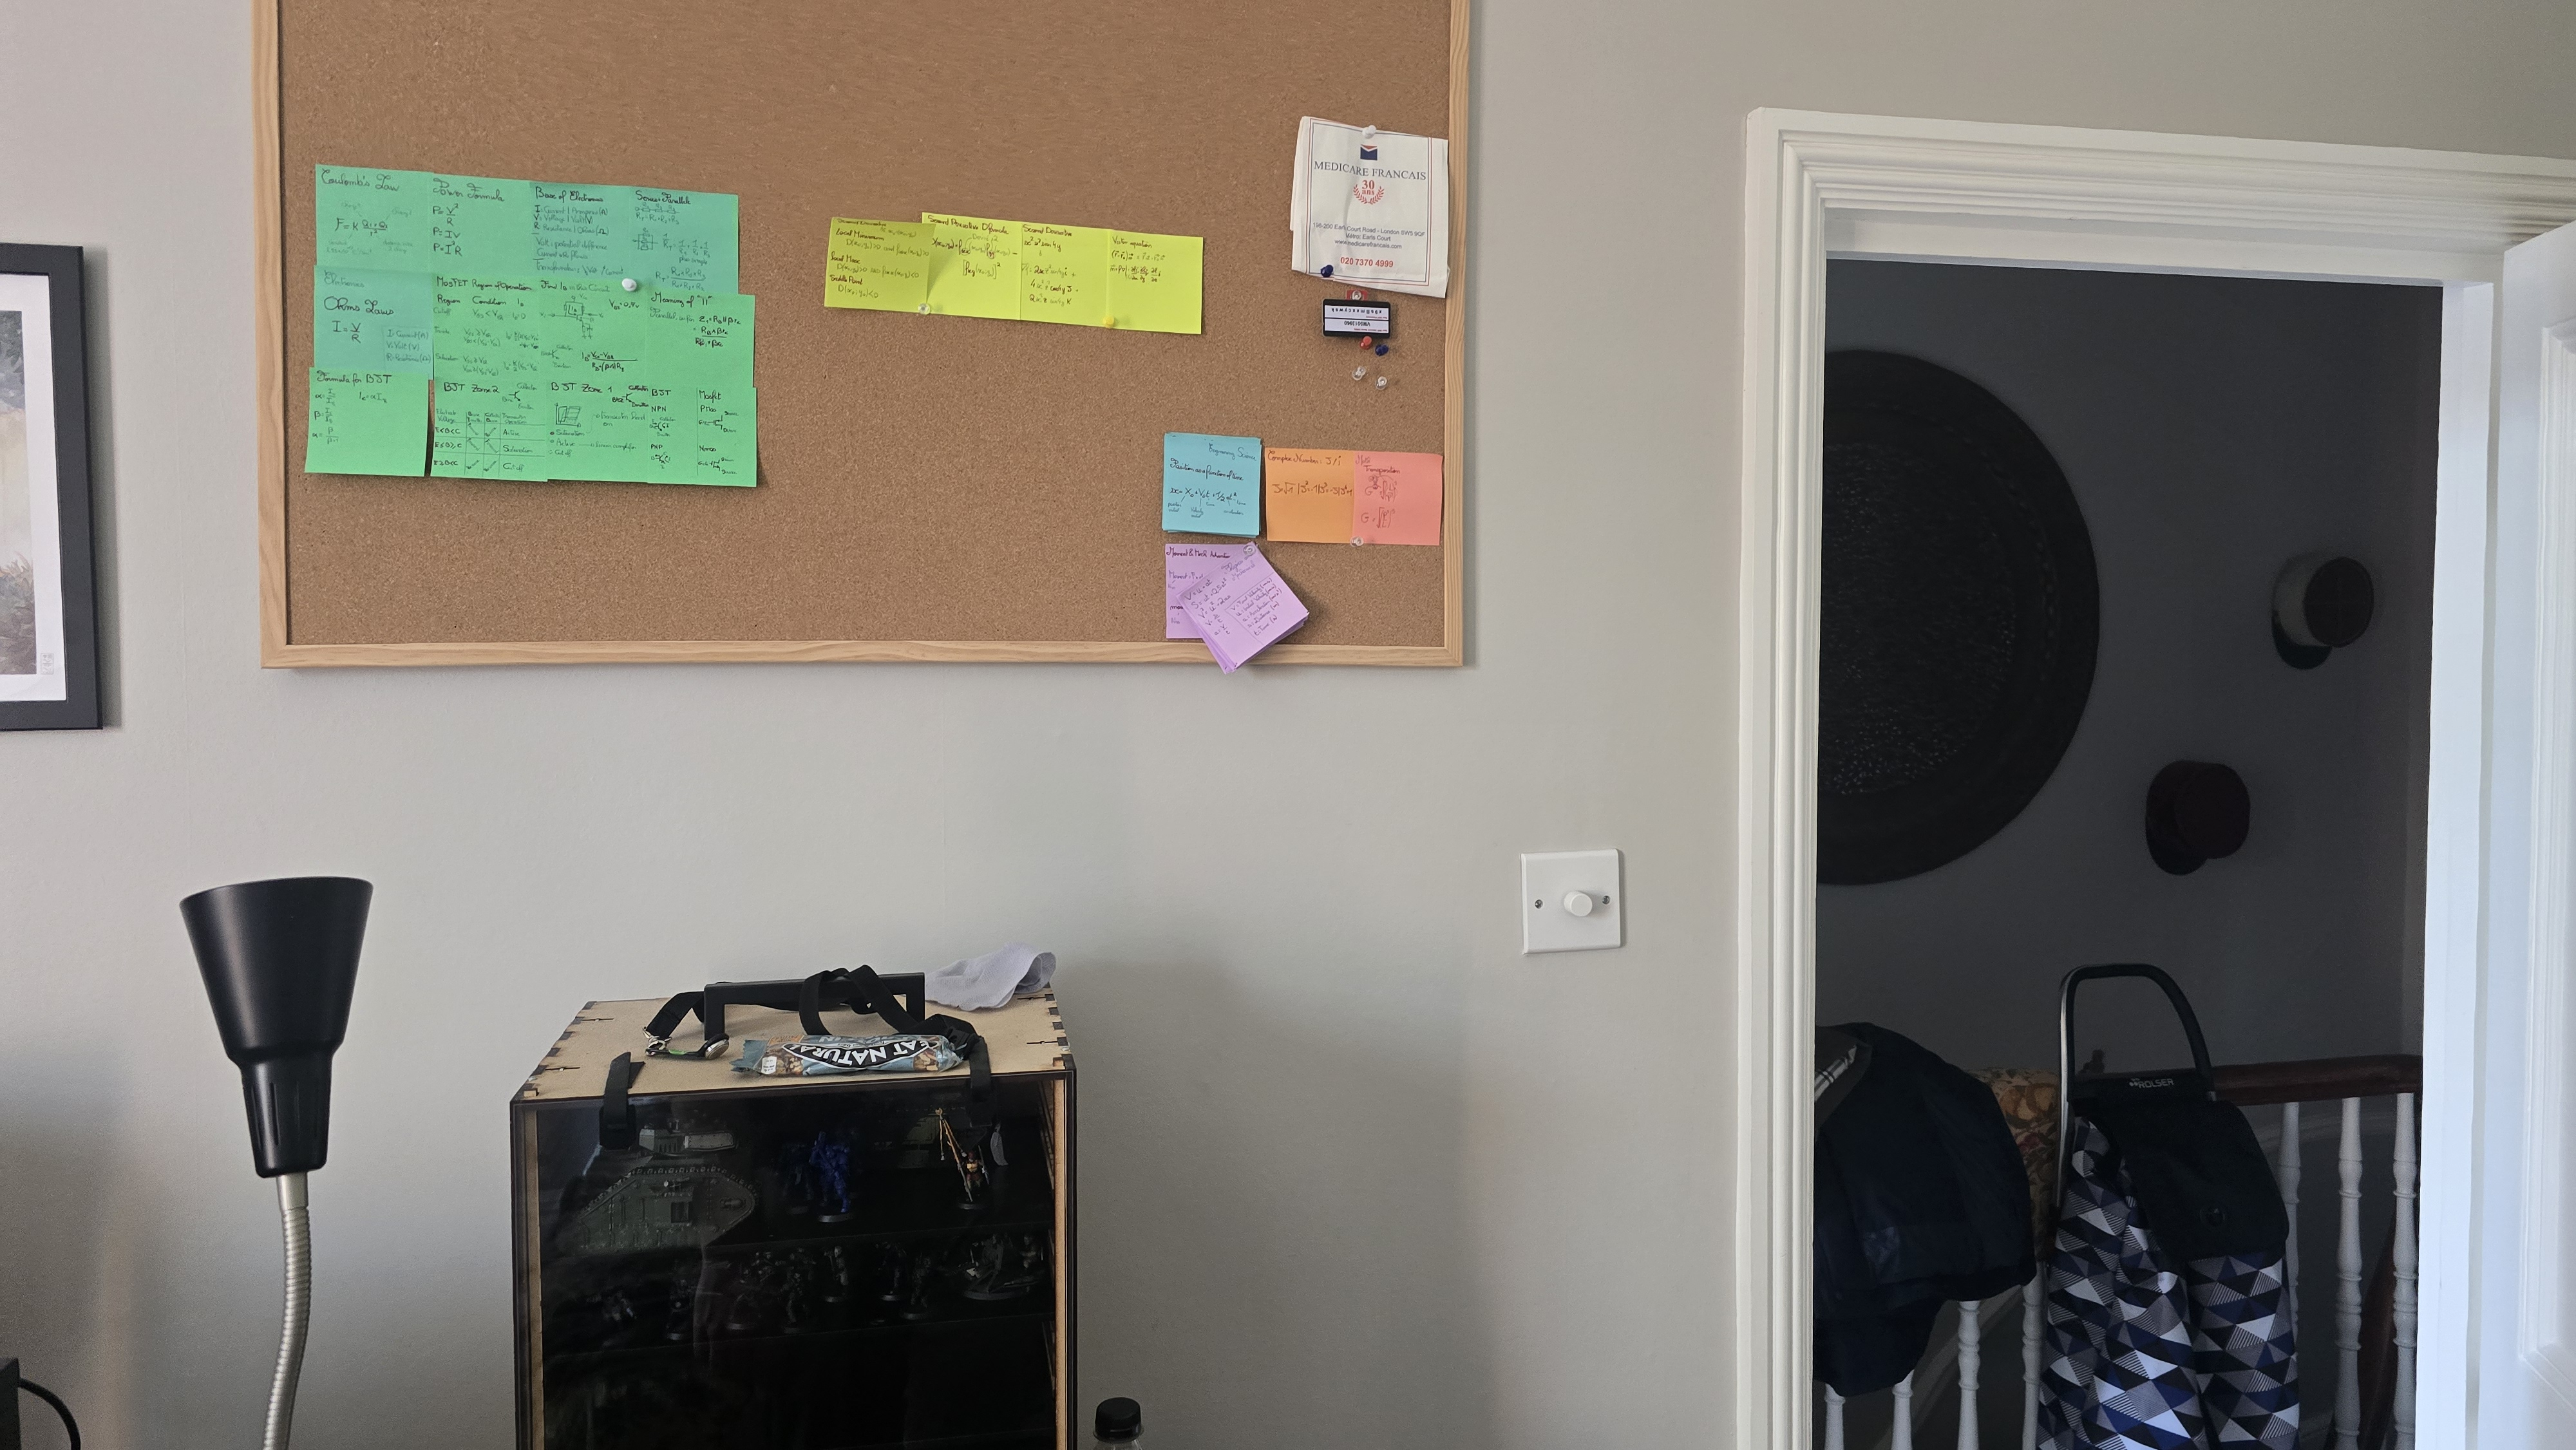
\includegraphics[width=0.78\linewidth]{Pictures of Cork Board/1000299773.jpg}
\caption{Wider shot of P2's corkboard in situ next to the desk.}\label{fig:p2-cork3}
\end{figure}
\newpage
\subsubsection*{P4: live screen-share}\label{app:obs-p4}
\begin{itemize}[leftmargin=1.2em,itemsep=2pt]
    \item \textbf{Setting.} P4's own laptop, used in the interview
          room. Some initial fiddling to get screen-sharing into Teams
          before the demonstration began [P4~I4:267--275].
    \item \textbf{Sequence (data-analysis coursework).} Opened the
          module's Moodle page; pointed at a 10-April deadline. Said
          ``we'll do the data analysis one'' [P4~I4:281]. Read the
          course description in place: ``I think this is gas
          turbines\dots\ they mentioned it was an AI task. Conveniently,
          they outlined the tasks there'' [P4~I4:283]. Demonstrated the
          \textbf{brief-driven task derivation} pattern: read the brief,
          glean the topic, follow the tasks linearly one-by-one
          [P4~I4:287]. Mentioned the work was expected in a
          \textbf{Jupyter notebook} [P4~I4:295].
    \item \textbf{Sequence (electronics, exam module).} Switched
          modules to an electronics past paper. ``They had all their
          tutorials listed, so usually I just go through the tutorials
          and do the tutorials, and then attempt the mock paper''
          [P4~I4:301]. Located the mock paper; was unsure whether
          worked solutions were appended [P4~I4:301]. Stated the
          \textbf{solutions-on-second-screen} pattern.
    \item \textbf{Tools visible / referenced.} Browser (Moodle);
          implicit reference to Jupyter. iPad folder hierarchy
          (subject $\rightarrow$ exam $\rightarrow$ topic) was
          \emph{referenced} but not opened on screen [P4~I4:255].
    \item \textbf{Verbal description (mid-walkthrough).} Worked-example
          preference: ``It gives you a thought process to
          follow\dots\ `this is the way you should think of this
          module'.'' [P4~I4:309]. AI is last-resort: ``Usually only
          when I can't figure it out\dots\ I usually try and find a
          tutorial that's as close to the questions as possible and
          follow the reasoning for that.'' [P4~I4:313]. Past-paper
          cascade: tutorial $\rightarrow$ past-paper $\rightarrow$
          group call [P4~I4:317]. YouTube use: ``not usually about
          solving problems\dots\ for understanding the topic''
          [P4~I4:325--329]. Cascade: lecture $\rightarrow$ topic
          $\rightarrow$ YouTube $\rightarrow$ tutorial [P4~I4:341].
    \item \textbf{Last-session refresher (described, not
          demonstrated).} Referenced the iPad folder structure and the
          habit of keeping the previous session's notes on a different
          monitor as a refresher [P4~I4:255--259].
    \item \textbf{What was not observed.} No live opening of the iPad
          notes; no AI tool opened; no group-call activity.
\end{itemize}

\subsubsection*{P3: verbal scenario walkthrough only}\label{app:obs-p3}
\begin{itemize}[leftmargin=1.2em,itemsep=2pt]
    \item \textbf{Setting.} No computer present; no physical artefact
          shown. The walkthrough was conducted entirely verbally, with
          the interviewer prompting ``imagine the exam is in two days,
          walk me through your thought process'' [P3~I3:284]. Less
          in-depth than P1, P2 or P4: the interviewer largely led the
          cascade and P3 confirmed steps rather than narrating them at
          length.
    \item \textbf{Sequence described.} Moodle $\rightarrow$ tutorials
          $\rightarrow$ previous years' work $\rightarrow$ mock paper
          as diagnostic [P3~I3:288--292]. On a poor mock score, focus
          narrows to the weak topic (``control systems'')
          [P3~I3:296--304]; tutorial sheet revisited and fed into AI
          for additional questions [P3~I3:308]; YouTube invoked as a
          third-party recall aid [P3~I3:312]. Cycle repeats with a
          second mock; target ${\sim}65$\%, push higher if time allows
          [P3~I3:316--322]. Readiness signal: tutorials and tools
          ``all done'' by the Sunday before the exam
          [P3~I3:326--334].
    \item \textbf{Tools referenced (not opened).} Moodle, AI, YouTube.
    \item \textbf{What was not observed.} No screen interaction, no
          artefact, no live tool use.
\end{itemize}

% ============================================================
% GENAI USAGE LOG
% ============================================================
\newpage
\section{GenAI Usage Log}\label{app:genai}

The following table documents all use of Generative AI tools during the
preparation of CW2 materials, including prompts/inputs, outputs and uses.

\vspace{0.5em}
\noindent
\setlength{\emergencystretch}{3em}
\begin{longtable}{@{}>{\raggedright\arraybackslash}p{1.8cm}>{\raggedright\arraybackslash}p{2.8cm}>{\raggedright\arraybackslash}p{4.5cm}>{\raggedright\arraybackslash}p{4.5cm}@{}}
\toprule
\textbf{Date} & \textbf{Tool} & \textbf{Prompt/Input} & \textbf{Output \& Use} \\
\midrule
\endhead
2026-04-23
& Claude Opus 4.7 (Claude Code CLI)
& \texttt{start with a skeleton for pt2, and sections to logically
  work through.}
& Created \texttt{part-2/pt2.tex} as an empty skeleton mirroring the
  CW2 brief structure (cover page, User Research / Design /
  Usability Testing sections, References, Appendices and this
  GenAI log) and an empty \texttt{references.bib}. All section
  content left as TODO comments for the student to author. \\
\midrule
2026-04-24
& Claude Opus 4.7 (Claude Code CLI)
& \texttt{Write this to a md file for context for me.}
& Wrote \texttt{part-2/ROADMAP.md} as a personal working document
  (not a submission deliverable) capturing locked design direction,
  the planned wireframe journey, an analysis pipeline outline, a
  phase-by-phase checklist and a marking-weight table. No analytic
  content (findings, persona, wireframes) was generated. \\
\midrule
2026-04-26
& Claude Opus 4.7 (Claude Code CLI)
& \texttt{correct the onedrive folder url properly please.} +
  \texttt{can you take a look at my pt2?} + \texttt{clean all
  these up.}
& Cover-page OneDrive placeholder replaced with a clean
  \texttt{\textbackslash href} link. Cleanup pass on
  \texttt{pt2.tex} (no analytic content added): fixed a stray
  backtick in the URL; escaped a bare \texttt{\&} in \S1.1;
  repointed two undefined \texttt{\textbackslash ref} targets;
  added a \texttt{Research Materials} appendix as the resolution
  target for the Qualtrics-screener cite; deleted four duplicate
  empty subsection stubs in \S1.2; added a Braun \& Clarke 2006
  entry to \texttt{references.bib} and converted the inline
  citation to \texttt{\textbackslash textcite\{braun2006\}} so
  the bibliography is populated. \\
\midrule
2026-04-26
& Claude Opus 4.7 (Claude Code CLI)
& \texttt{which template for figjam?}
& Gave advice regarding which default template to use in FigJam. ``Affinity mapping with sticky notes for clustering''. \\
\midrule
2026-04-27
& Claude Opus 4.7 (Claude Code CLI)
& \texttt{Is the affinity mapping from the 4 interviews accurate?
  Doublecheck (and take a look at figjam.pdf).} 
& Cross-checked every sticky in
  \texttt{part-2/\allowbreak figjam-stickies.md} against
  \texttt{Interview1--4.md} and against the rendered
  \texttt{figjam.pdf}. Reported back the (mostly accurate)
  attribution, plus three concrete bugs: a duplicated sticky
  (\emph{peer-asking only at exam season (P1)}) appearing in
  both T1 and T4, a typo (\emph{personal coding} $\to$
  \emph{personal colour-coding}) and 5~T1 stickies present in
  the .md but missing from the rendered board. Applied the
  duplicate-removal and typo fix to
  \texttt{figjam-stickies.md}; the figjam canvas itself
  was not modified. \\
\midrule
2026-05-01
& Claude Opus 4.7 (Claude Code CLI)
& \texttt{Hey! I added my wireframes in Wireframes/. I would like
  you to polish the annotations.}
& In \texttt{pages.jsx}: tightened the per-screen callout copy
  (kept all participant, requirement and heuristic citations
  verbatim), added \texttt{pins} arrays for each of the seven
  screens specifying CSS-selector targets and column side, and
  added a \texttt{usePinLayout} React effect that resolves those
  selectors against the rendered phone, places the numbered pins
  on the screen edge and draws SVG bezier leader lines into the
  matching spec cards. Minor copy fix in one of the screens 
  (literal newline in the briefing-card module string). Annotation
  substance, screen content and requirements are unchanged. \\
\midrule
2026-05-02
& Claude Opus 4.7 (Claude Code CLI)
& \texttt{Let's clean all of the gendered language up.}
& Searched all CW2 source files (Wireframes JSX, \texttt{analysis.md},
  \texttt{pt2.tex}) for gendered pronouns referring to study
  participants, where the gender was inferred during writing rather
  than disclosed by the participants themselves (P2 specifically
  asked to be referred to by a pseudonym during consent). Replaced
  inferred \emph{he/she/him/his} with the gender-neutral
  \emph{they/them/their}, with verb-form adjustments where needed
  (e.g.\ ``every time he passes'' $\to$ ``every time they pass'';
  ``she currently has'' $\to$ ``they currently have''). Three
  edits in \texttt{Wireframes/pages.jsx} (Screen~01 evidence,
  Screen~02 intro, Screen~07 evidence). Twelve edits in
  \texttt{part-2/analysis.md} (P1 walkthrough setting, P2
  walkthrough artefact descriptions, P1 group-study summary, P2
  wall-plank descriptions, pull-quote attribution). Verbatim
  participant quotes referring to third parties (the participant's
  mother) were preserved unchanged in the analysis tables
  (\texttt{analysis.md:237, 314}): rewriting verbatim research
  data would misrepresent the source. No changes to interview
  transcripts (\texttt{Interview1--4.md}). \\
\midrule
2026-05-02
& Claude Opus 4.7 (Claude Code CLI)
& \texttt{fix the latex compilation warnings/errors.}
& Cleared all 464 underfull/overfull warnings and the duplicate
  \emph{page.1}/\emph{page.2} hyperref destination warnings from
  \texttt{pt2.log}, with no changes to substantive prose. Five
  edits to \texttt{pt2.tex}: (1)~replaced the \emph{titlepage}
  environment (which silently resets the page counter to~1 after
  its end, producing duplicate hyperref \emph{name\{page.N\}}
  anchors) with a plain \emph{center} environment plus a
  \emph{newpage} and \emph{tableofcontents}; (2)~added the
  \emph{array} and \emph{microtype} packages; (3)~switched the
  GenAI longtable column spec from justified \emph{p\{\}} columns
  to \emph{raggedright}-prefixed columns to stop justified narrow
  columns producing $\sim$460 underfull hboxes around the many
  \emph{texttt} tokens; (4)~added a 3em \emph{emergencystretch}
  before the longtable; (5)~inserted \emph{allowbreak} after
  slashes inside the four longest \emph{texttt} file paths
  (\texttt{Coursework/\allowbreak Wireframes/\allowbreak styles.css},
  \texttt{Coursework/\allowbreak Wireframes/\allowbreak screens.jsx},
  \texttt{part-2/\allowbreak figjam-stickies.md} $\times$2) so TeX
  can break them across lines. Verified with \emph{pdflatex +
  biber + pdflatex} $\times$2: zero warnings, zero errors. \\
\midrule
2026-05-03
& Claude Opus 4.7 (Claude Code CLI)
& \texttt{Make my pt2.tex compile properly please ;)}
& Diagnosed the \texttt{pt2.log} fatal error
  (\emph{Extra alignment tab has been changed to \textbackslash cr} at
  l.1713): the \emph{2026-04-26} row in this GenAI longtable was
  missing its terminating \texttt{\textbackslash\textbackslash} and
  \texttt{\textbackslash midrule}, so the next row's first \texttt{\&}
  was parsed as a 5th column in the previous row. Added the missing
  row terminator and changed the straight quotes around
  \emph{Affinity mapping with sticky notes for clustering} to LaTeX
  curly quotes. Reran \emph{pdflatex + biber + pdflatex}: PDF builds
  to 57 pages, the cascade of 25 \emph{undefined reference} warnings
  (which were a knock-on of the aborted first pass not writing labels
  to \texttt{.aux}) cleared on its own. \\
\midrule
\bottomrule
\end{longtable}
\end{document}